% The preamble has been dumped out as out/presentationpreamble.fmt file. You can recreate that file by
% xelatex -ini -jobname="pinholepreamble" -output-directory=out "&xelatex pinholepreamble.tex\dump"
% 
% To compile you need to load that binary file using -fmt option
% xelatex -fmt out/pinholepreamble.fmt -output-directory=out pinhole.tex
%\documentclass[10pt, compress]{beamer}
\usetheme{m}
 
 \usepackage{booktabs} % for better tables
 \usepackage{media9} % for includemedia i.e. videos
 \usepackage{xcolor} % for more colors
 \usepackage{hyperref} % for links
 \usepackage{cutwin} % text wrapped around figures
 \usepackage[backend=bibtex]{biblatex} % fancy citations
 \usepackage{ifthen}
 
\usepackage{tikz}
\usetikzlibrary{shadows,trees}
\usetikzlibrary{shapes,calc,backgrounds}
\usetikzlibrary{intersections}
\usepgfplotslibrary{dateplot}


%\tikzset{external/system call={xelatex -fmt out/pinholepreamble.fmt \tikzexternalcheckshellescape -shell-escape -halt-on-error -interaction=batchmode -jobname "\image" "\texsource"}}
%

% transparency
%\setbeamercovered{transparent=15}

\title{Pinhole camera}
\date{\today}
\author{Vikas Dhiman\\ David Johnson\\ Jason J Corso}
\institute{University of Michigan}
\bibliography{pinhole}

\begin{document}
\maketitle
\begin{frame}{Contents}
  % This slide will be removed later
  \tableofcontents
\end{frame}
% \begin{frame}{Sources}
%   \begin{itemize}
%     \item 
%       \url{http://www.exploratorium.edu/science_explorer/pringles_pinhole.html}
%     \item
%       \url{http://www.learner.org/workshops/sheddinglight/}
%   \end{itemize}
% \end{frame}
% \begin{frame}{Pinhole camera}
%   \centering
%   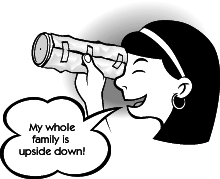
\includegraphics{media/girl_looks.png}
% \end{frame}

\section{About Light}
% Interesting notes/facts/videos about how human eye works.
% First camera "possibly" developed by ancient greeks and ancient Chinese.
% First documented description of a camera dates back to 1021 AD by a Arab physicist Ibn al-Haytham in his "Book of optics"
%%
%% How do you think our eyes work?
%% 
%% 
%% or 
%% 
%% 
% Rhetoric questions? Get kids involved
% What do kids think, how does eye/camera work?

\begin{frame}{How do you think our eyes work?}

  \begin{columns}
    \begin{column}{0.75\textwidth}
      \begin{itemize}
        \item
          Does the ``sight'' travel from our eyes to the object?\\
          \visible<2-> {\color{red}{Euclid other Greek believed so around 300 BC}\footfullcite{BBC:Let there be Light (2006)}}
        \item
          \color{black}{or the ``light'' travels from the object to our eyes?}\\
          \visible<3-> {\color{red}Modern scientists the believe so, and I have no reasons to question them.}
      \end{itemize}
    \end{column}
    \begin{column}{0.25\textwidth}
        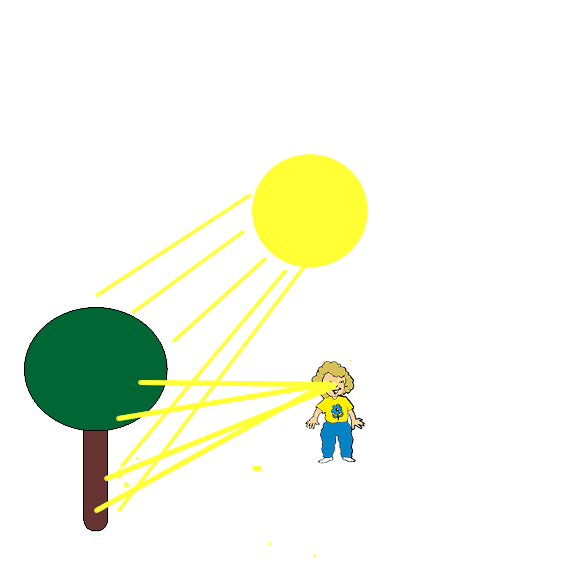
\includegraphics[width=\textwidth]{media/lghtmisc2.png}
    \end{column}
  \end{columns}
\end{frame}
% 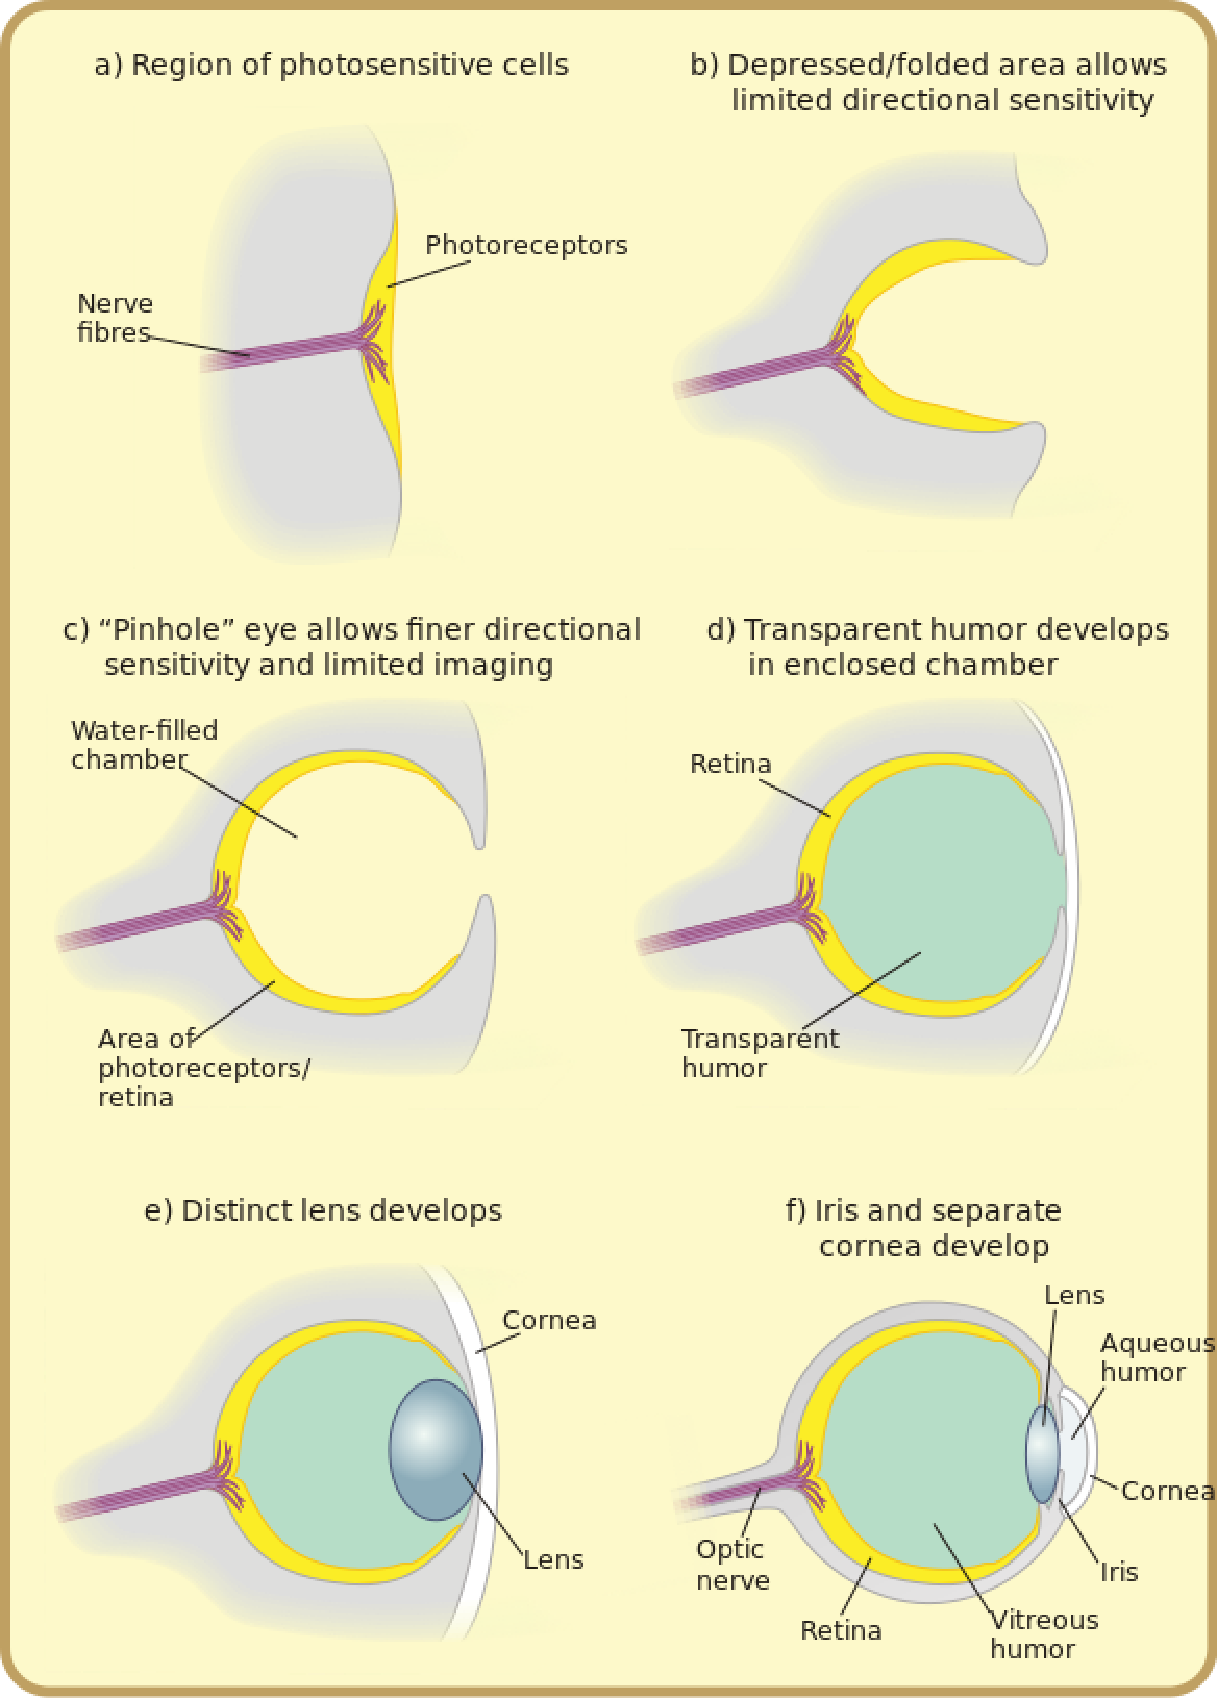
\includegraphics[width=\textwidth]{media/Diagram_of_eye_evolution.svg}
% \footfullcite{}

% \begin{frame}{What does it mean to see things?}
% 
% \end{frame}

\begin{frame}{What is light?}
  \begin{columns}
    \begin{column}{0.7\textwidth}
      \begin{itemize}
        \item Greek philosophers believed that sight was possible because of interaction of fire in eyes and in the sun.
        \item Euclid, a Greek philosopher, gave  us some particular insights about light.
      \end{itemize}
    \end{column}
    \begin{column}{0.3\textwidth}
      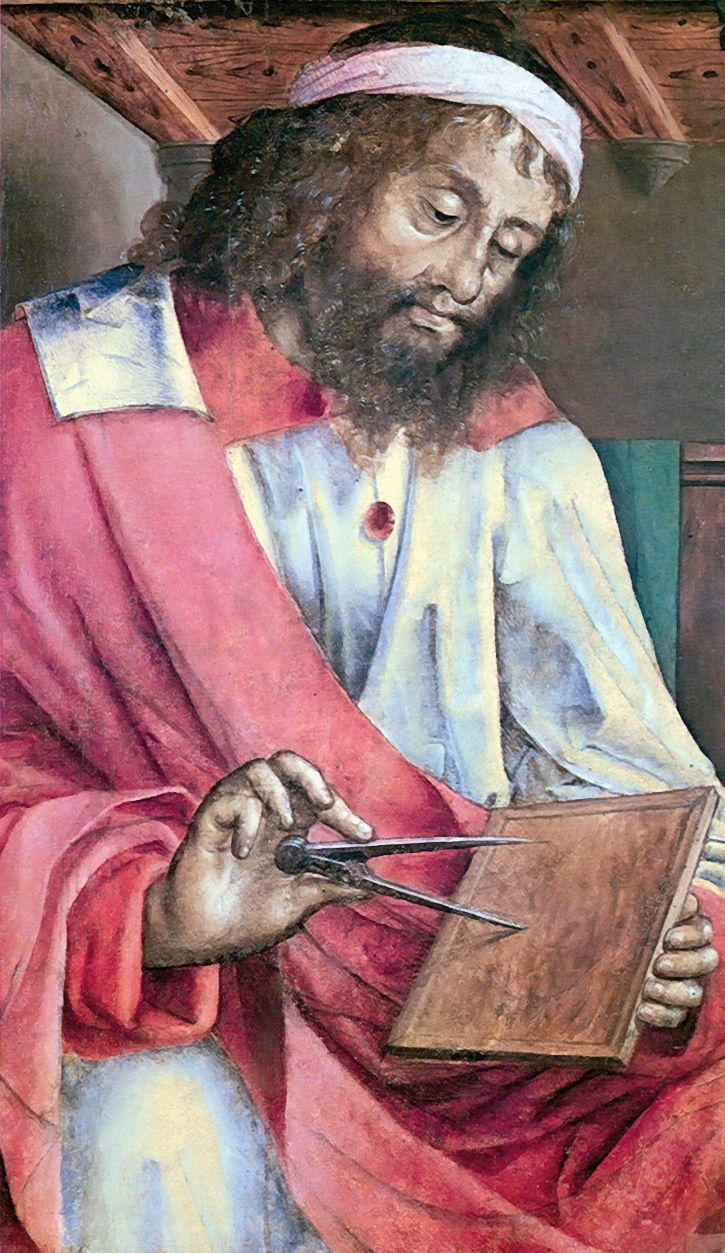
\includegraphics[width=\columnwidth]{media/Euklid.jpg}
    \end{column}
  \end{columns}
\end{frame}

\begin{frame}{Light travels in straight lines}
  \footfullcite{BBC:Let there be Light (2006)}
    \includemedia[label=euclid-straight-lines,
      width=\linewidth,height=0.6\linewidth, % 16:9
      activate=pageopen,
      addresource=media/euclid-straight-lines.mp4,
      flashvars={
        source=media/euclid-straight-lines.mp4
        &loop=false             % loop video
        &scaleMode=letterbox   % preserve aspect ratio while scaling the video
      }
    ]{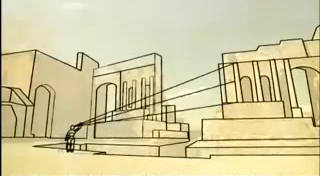
\includegraphics{media/euclid-straight-lines.png}}{VPlayer.swf}
\end{frame}

\begin{frame}{What is light?}
  Light is something that helps us see things. It travels in straight lines (well mostly!!).
\end{frame}

\section{Making a pinhole camera}
\frame{\tableofcontents[currentsection]}
\begin{frame}{Step 1}
  \begin{columns}
    \begin{column}{0.4\textwidth}
      Take a cup and scotch tape
    \end{column}
    \begin{column}{0.6\textwidth}
      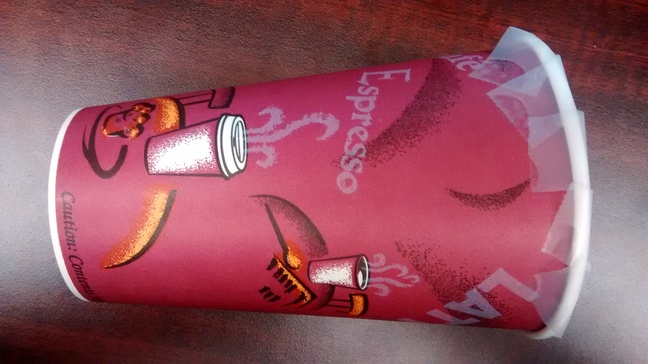
\includegraphics[width=\textwidth]{media/cup.jpg}\\
      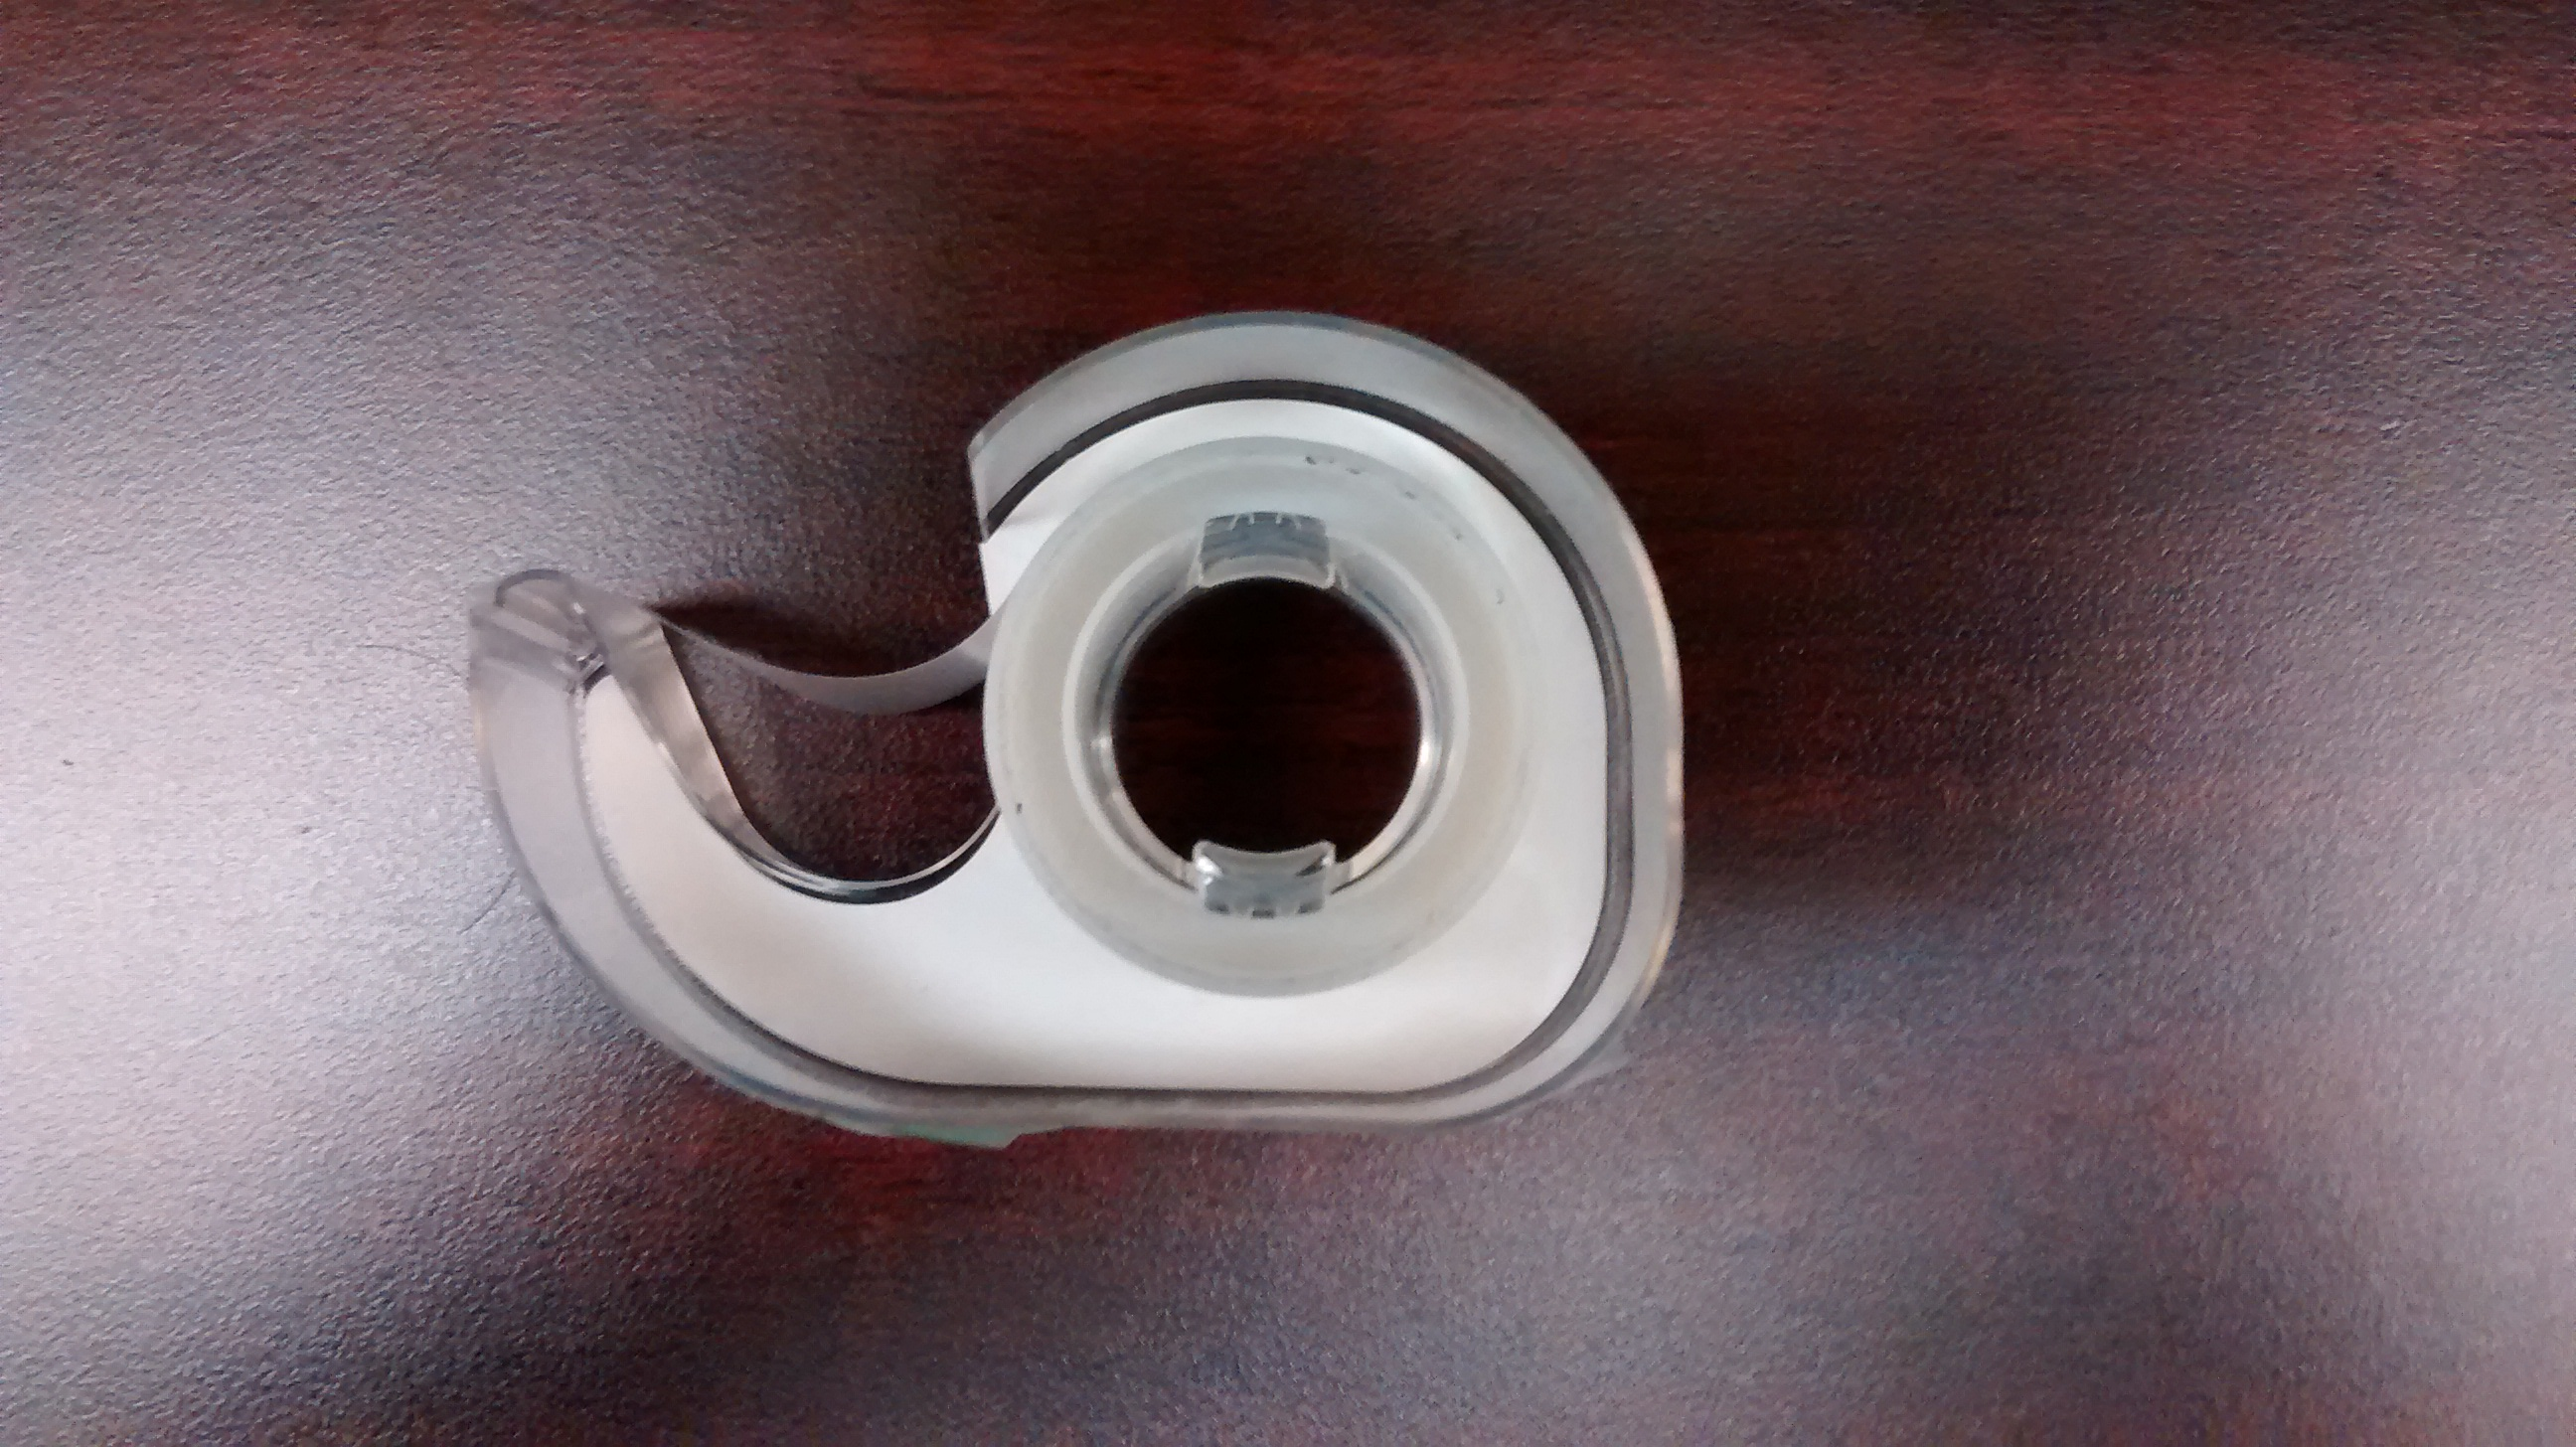
\includegraphics[width=\textwidth]{media/tape.jpg}
    \end{column}
  \end{columns}
\end{frame}

\begin{frame}{Step 2}
  \begin{columns}
    \begin{column}{0.6\textwidth}
      Cover the open end of cup using the scotch tape
    \end{column}
    \begin{column}{0.4\textwidth}
      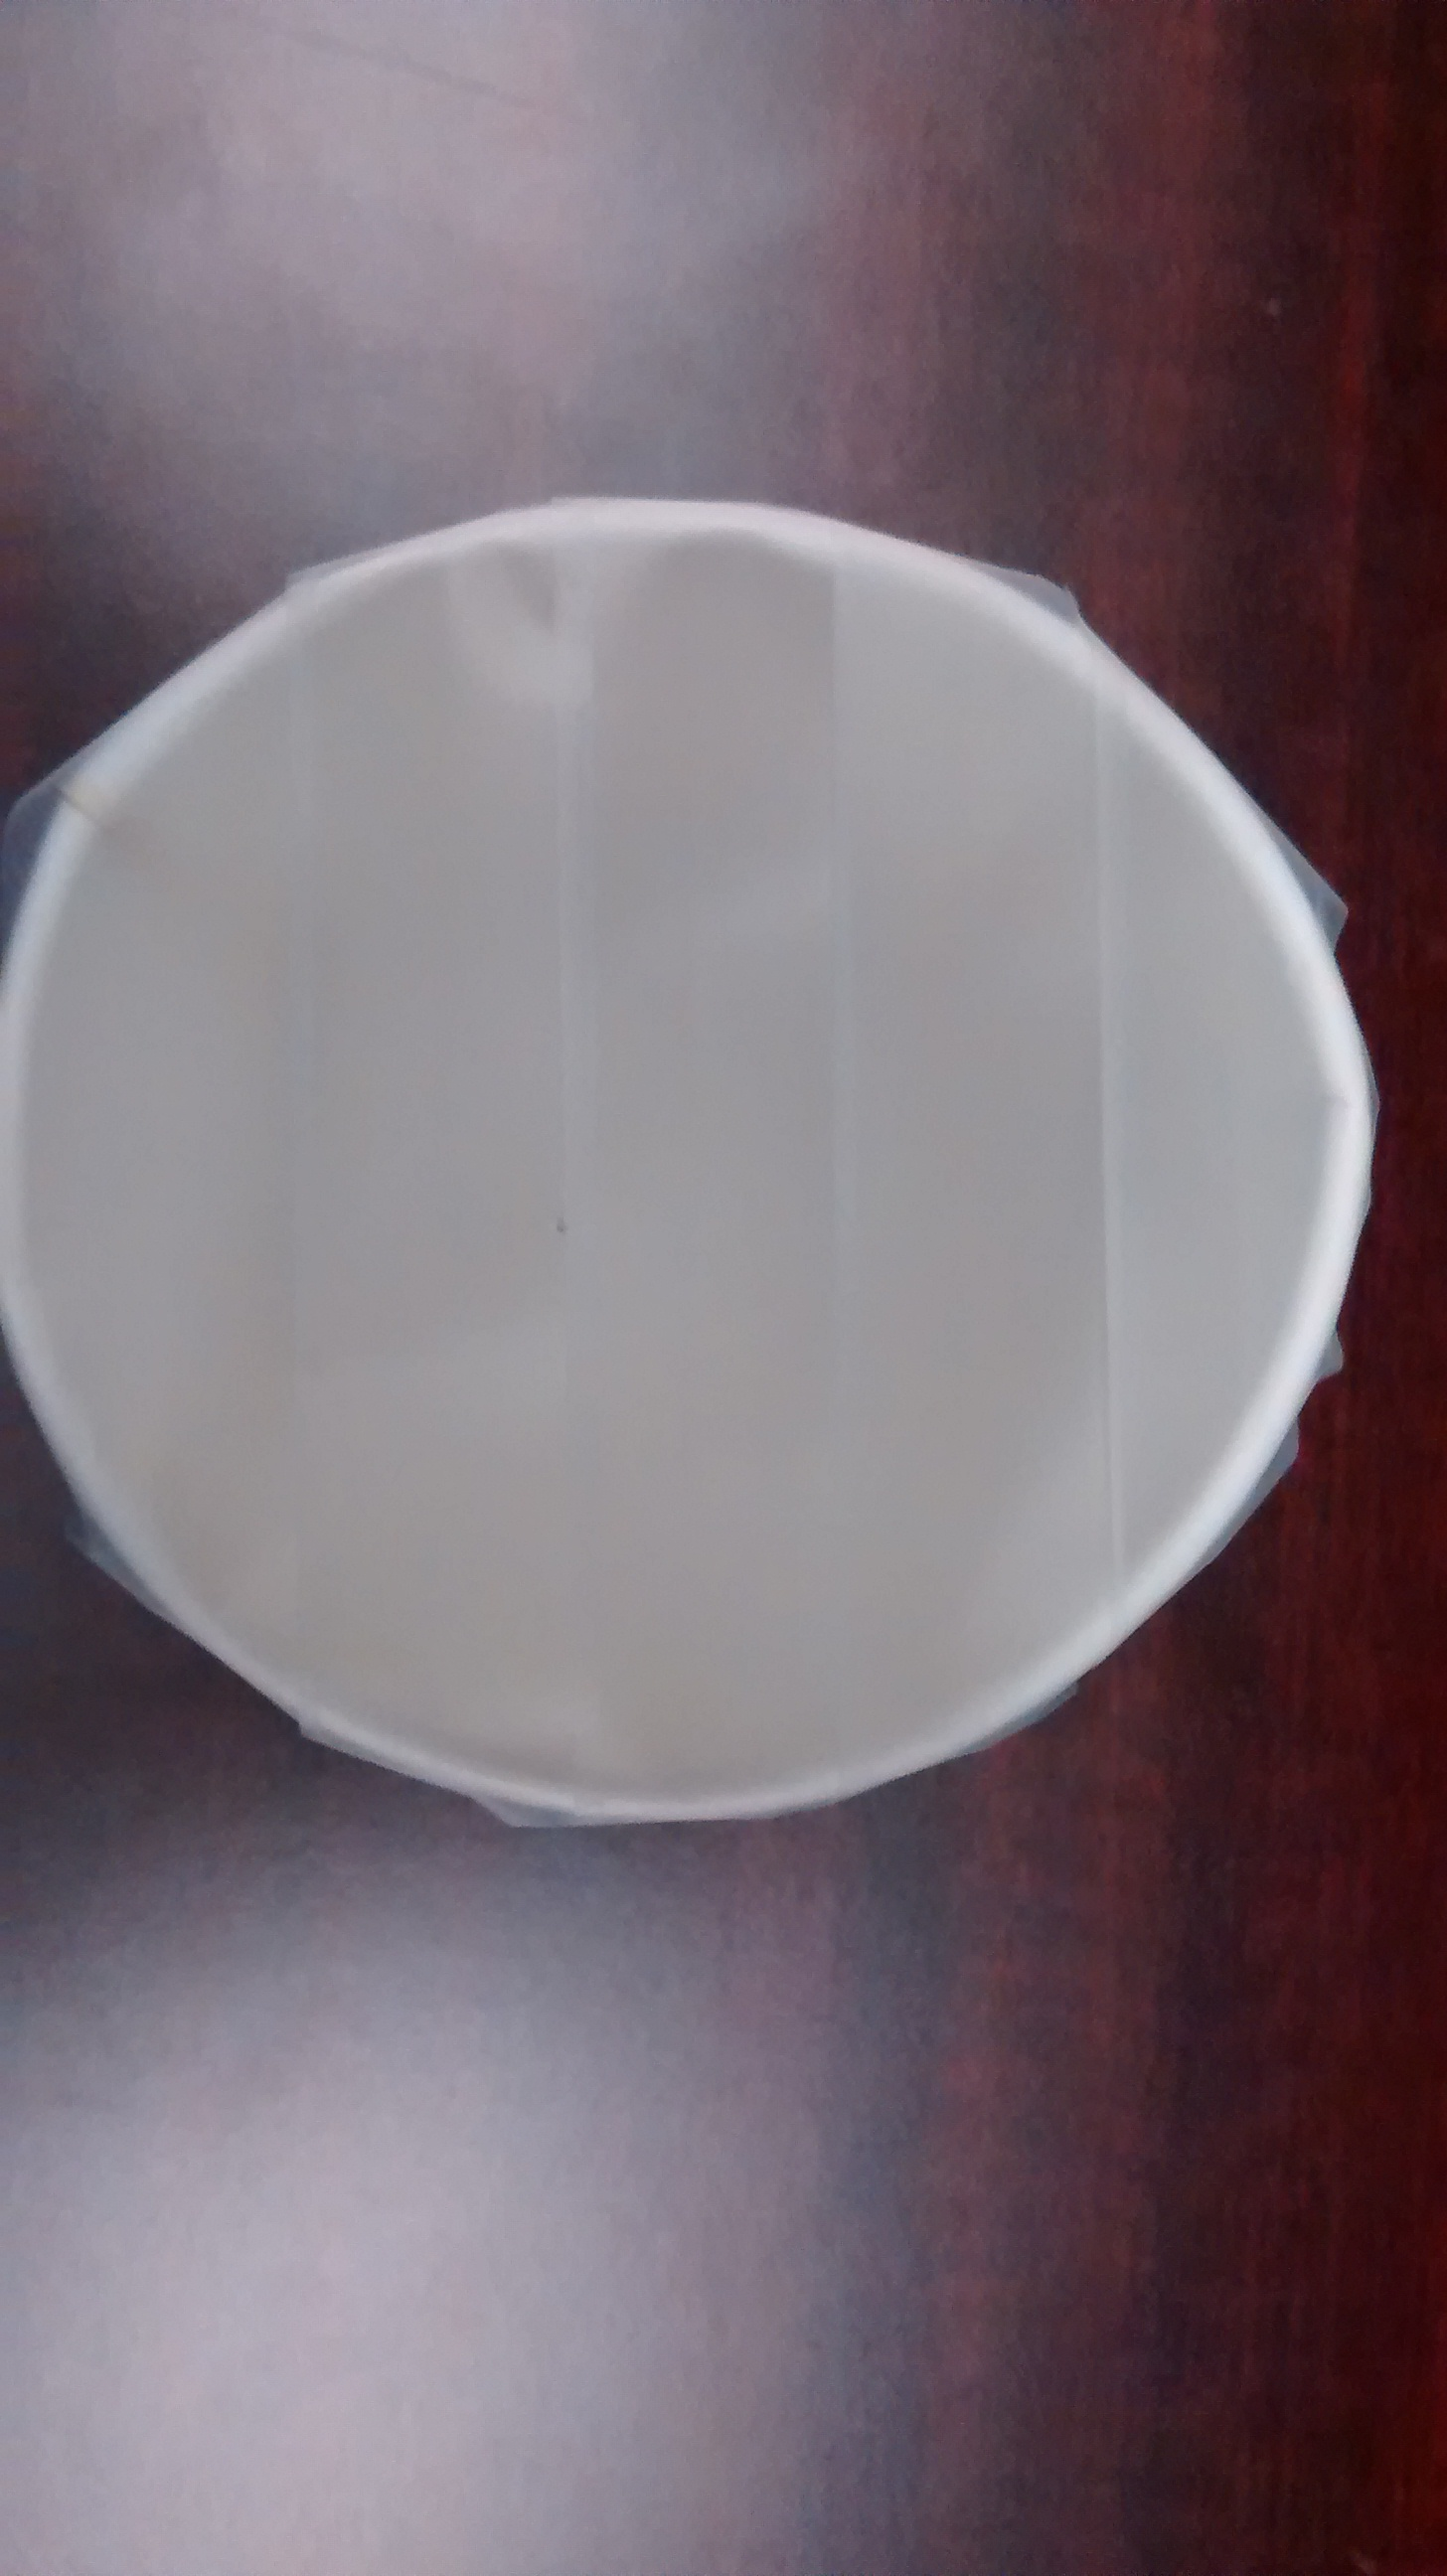
\includegraphics[width=\textwidth,trim=0 8in 0 4in,clip]{media/coveredlid2.jpg}\\
      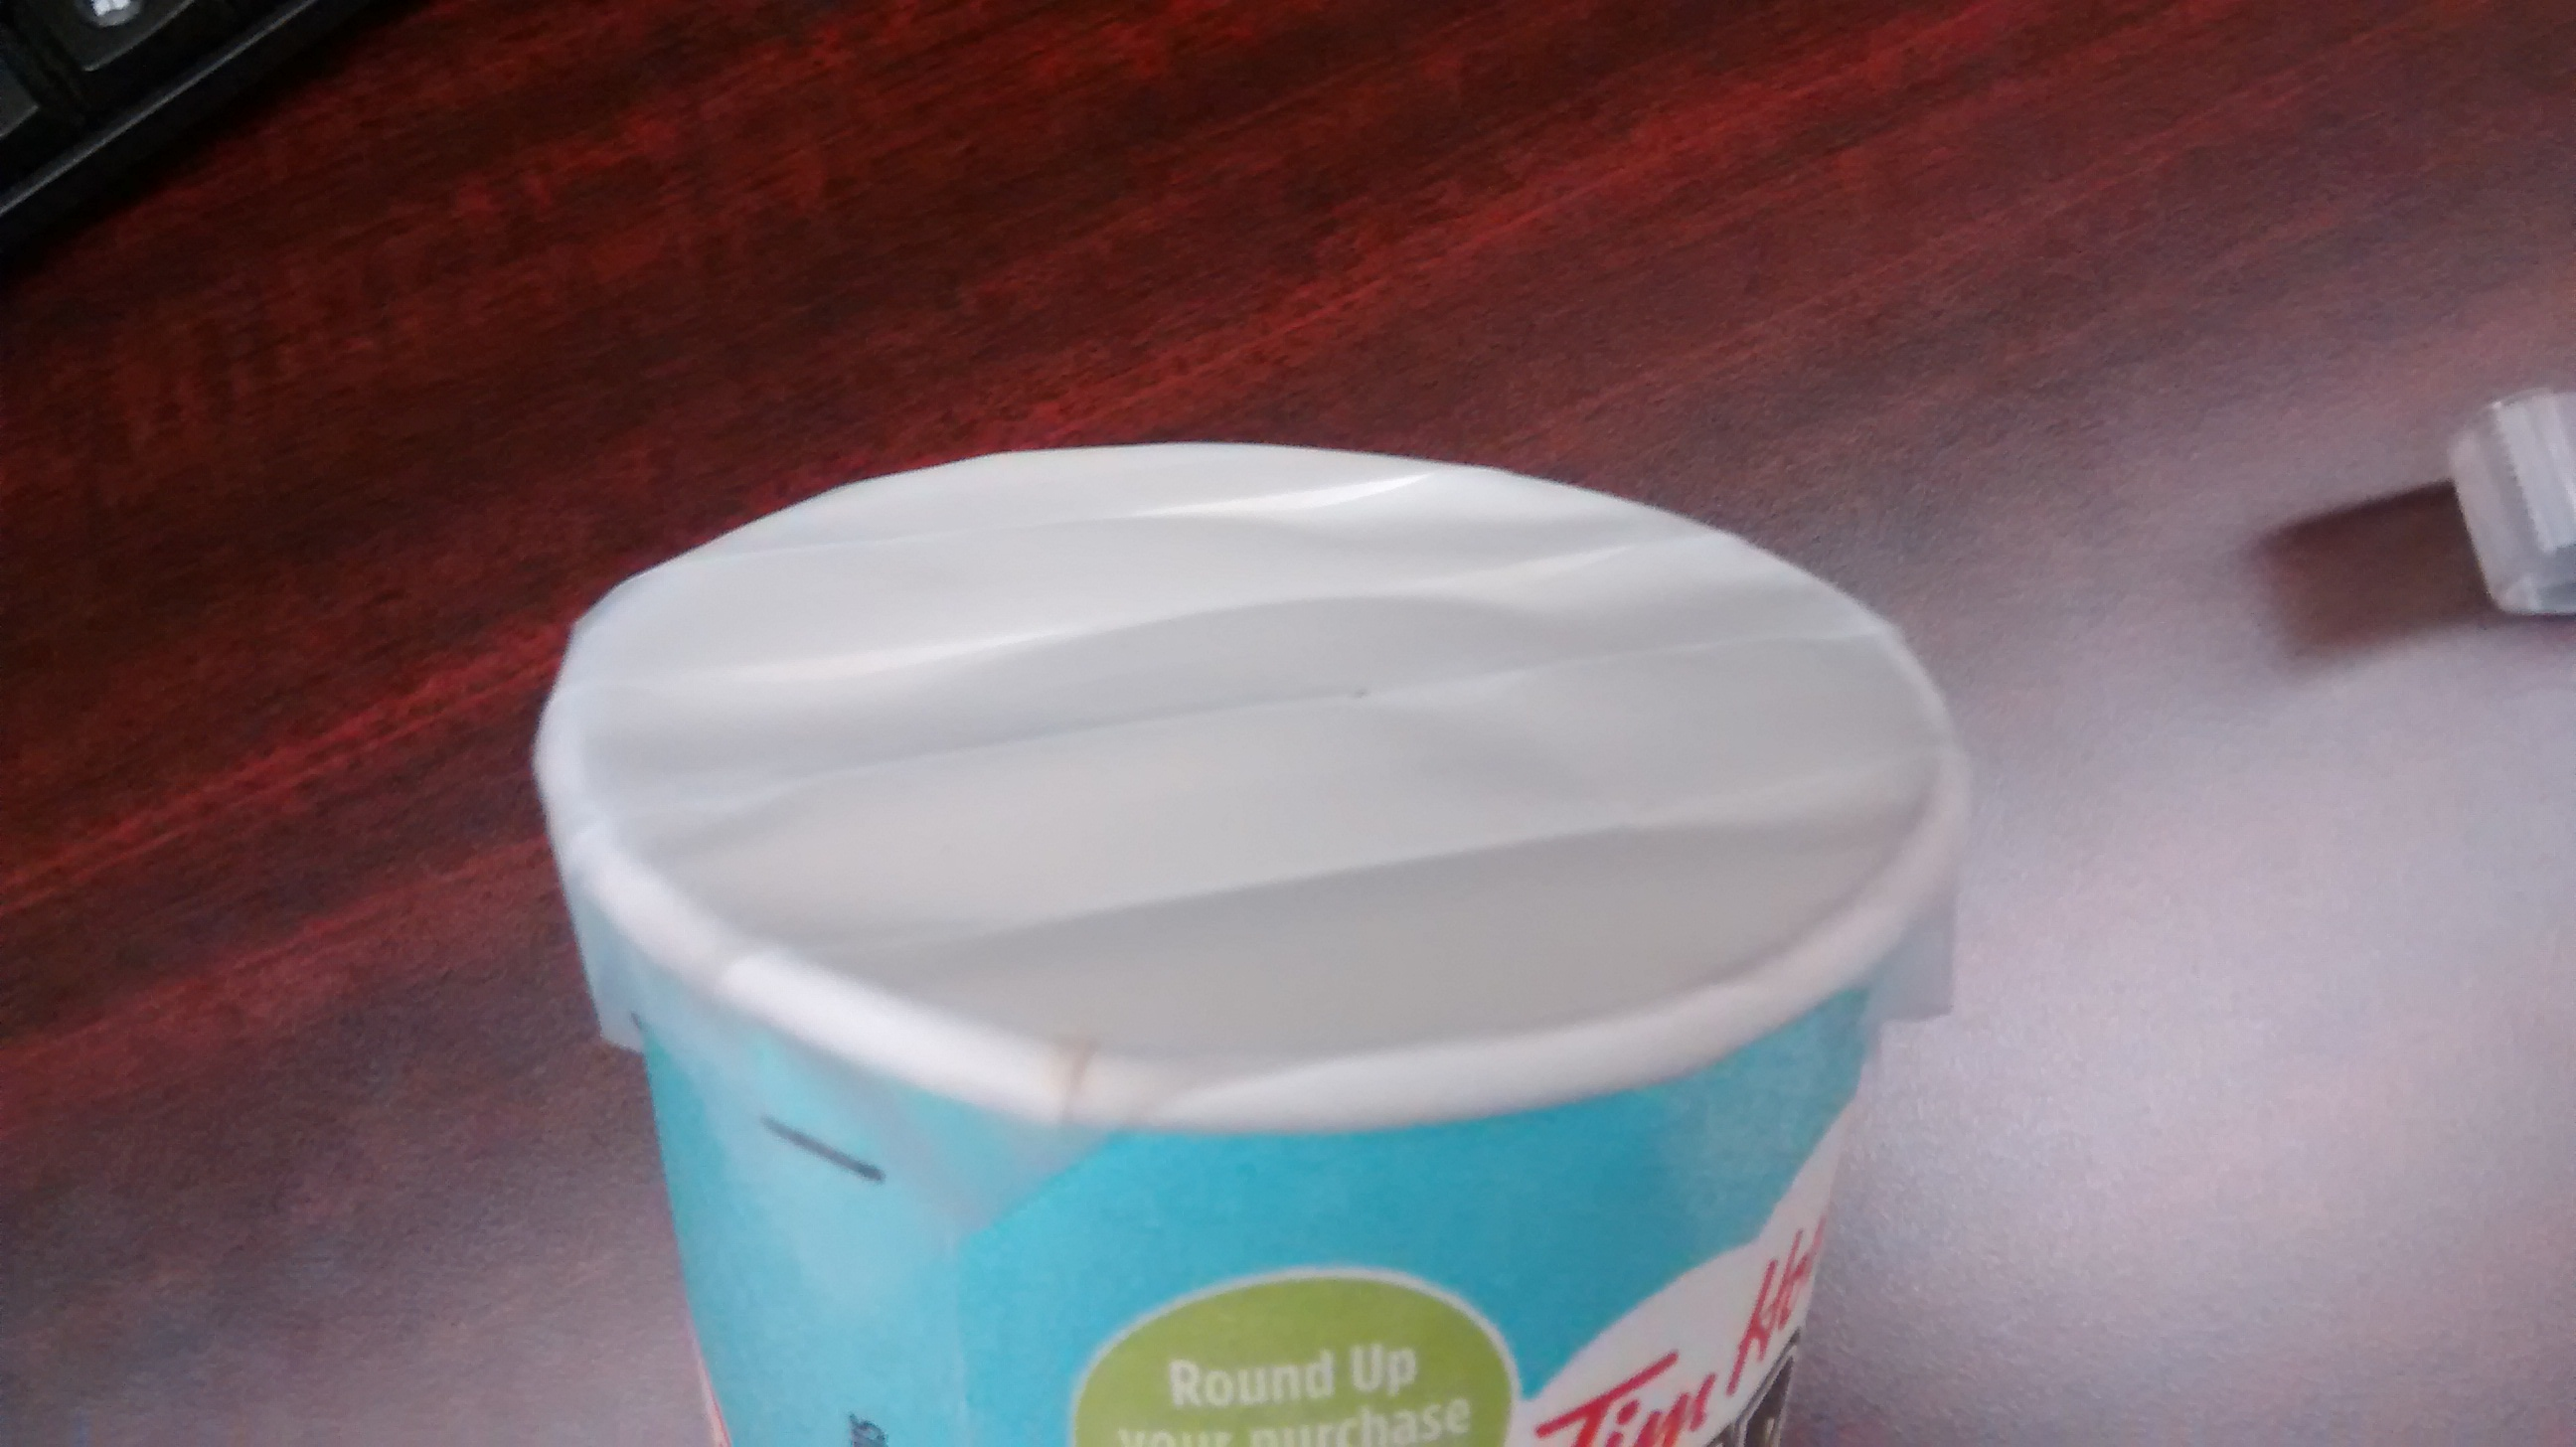
\includegraphics[width=\textwidth,trim=4in 0 4in 0,clip]{media/coveredlid1.jpg}
    \end{column}
  \end{columns}
\end{frame}

\begin{frame}{Step 3}
  \begin{columns}
    \begin{column}{0.6\textwidth}
      Cut a circular piece of construction paper to reinforce the cup base.
    \end{column}
    \begin{column}{0.4\textwidth}
      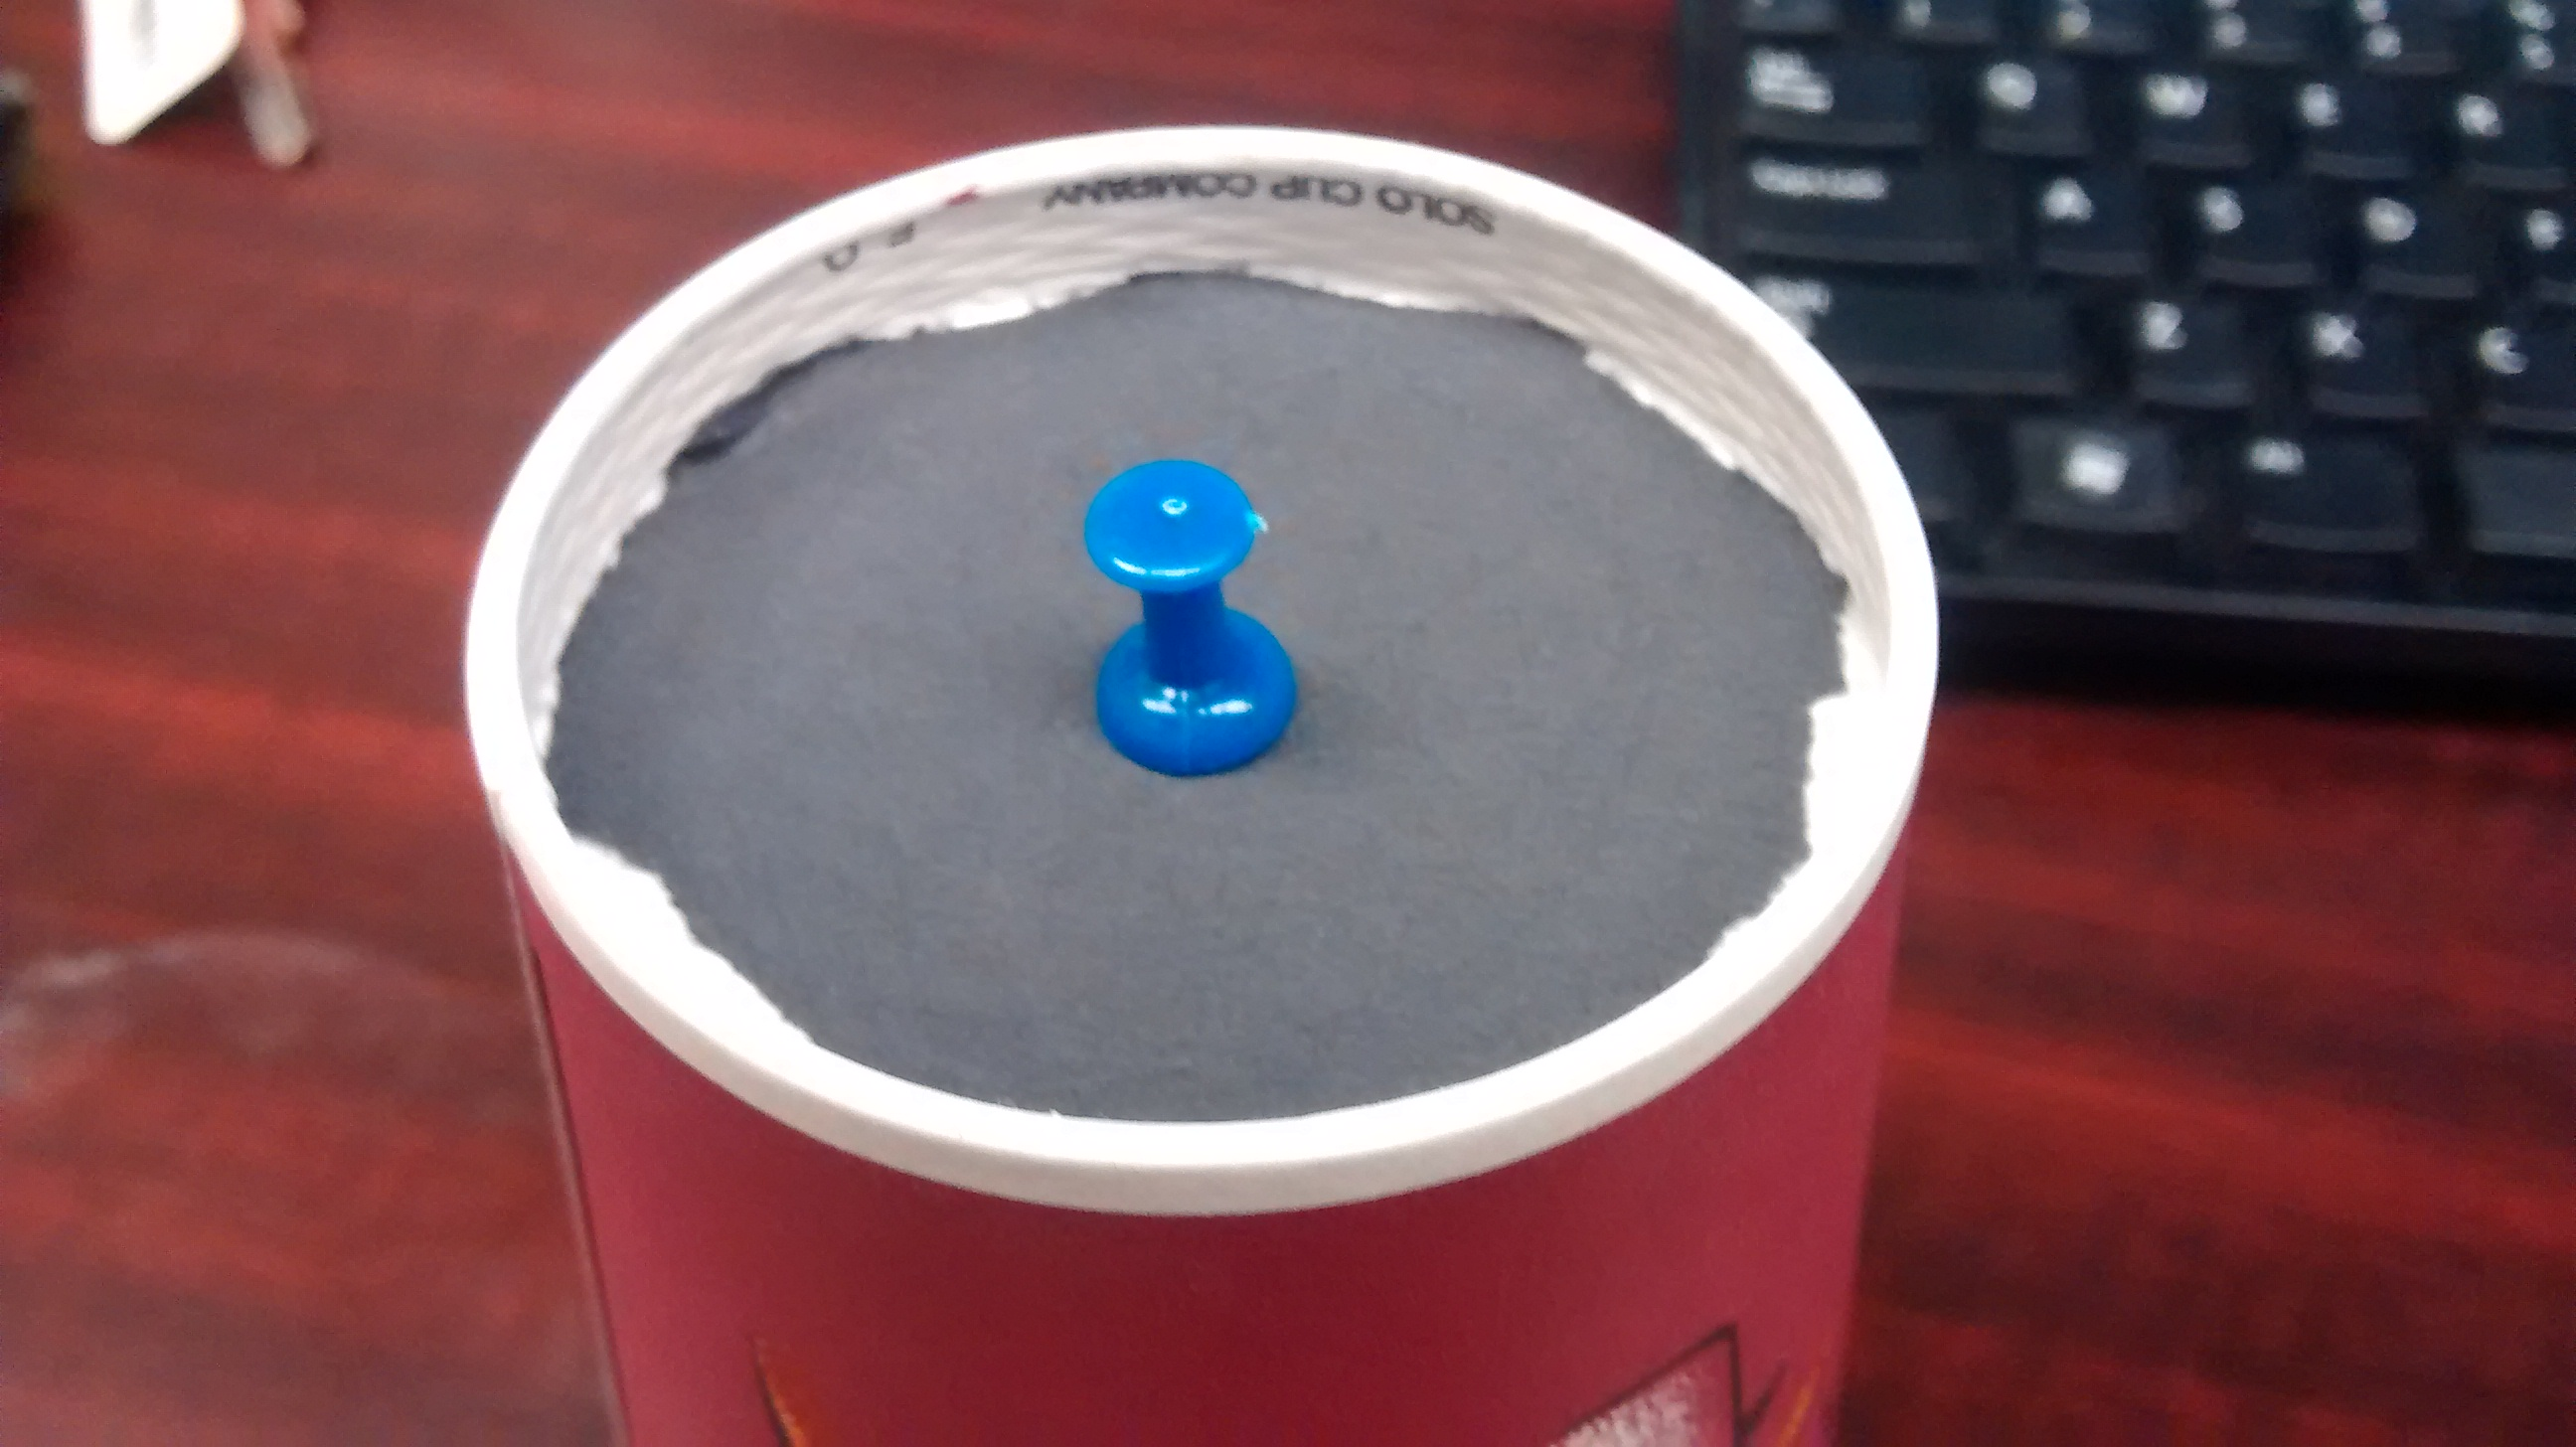
\includegraphics[width=\textwidth]{media/pushpin.jpg}
    \end{column}
  \end{columns}
  
\end{frame}

\begin{frame}{Step 4}
  \begin{columns}
    \begin{column}{0.6\textwidth}
      Pierce a pinhole through the closed end of the cup using a push pin
    \end{column}
    \begin{column}{0.4\textwidth}
      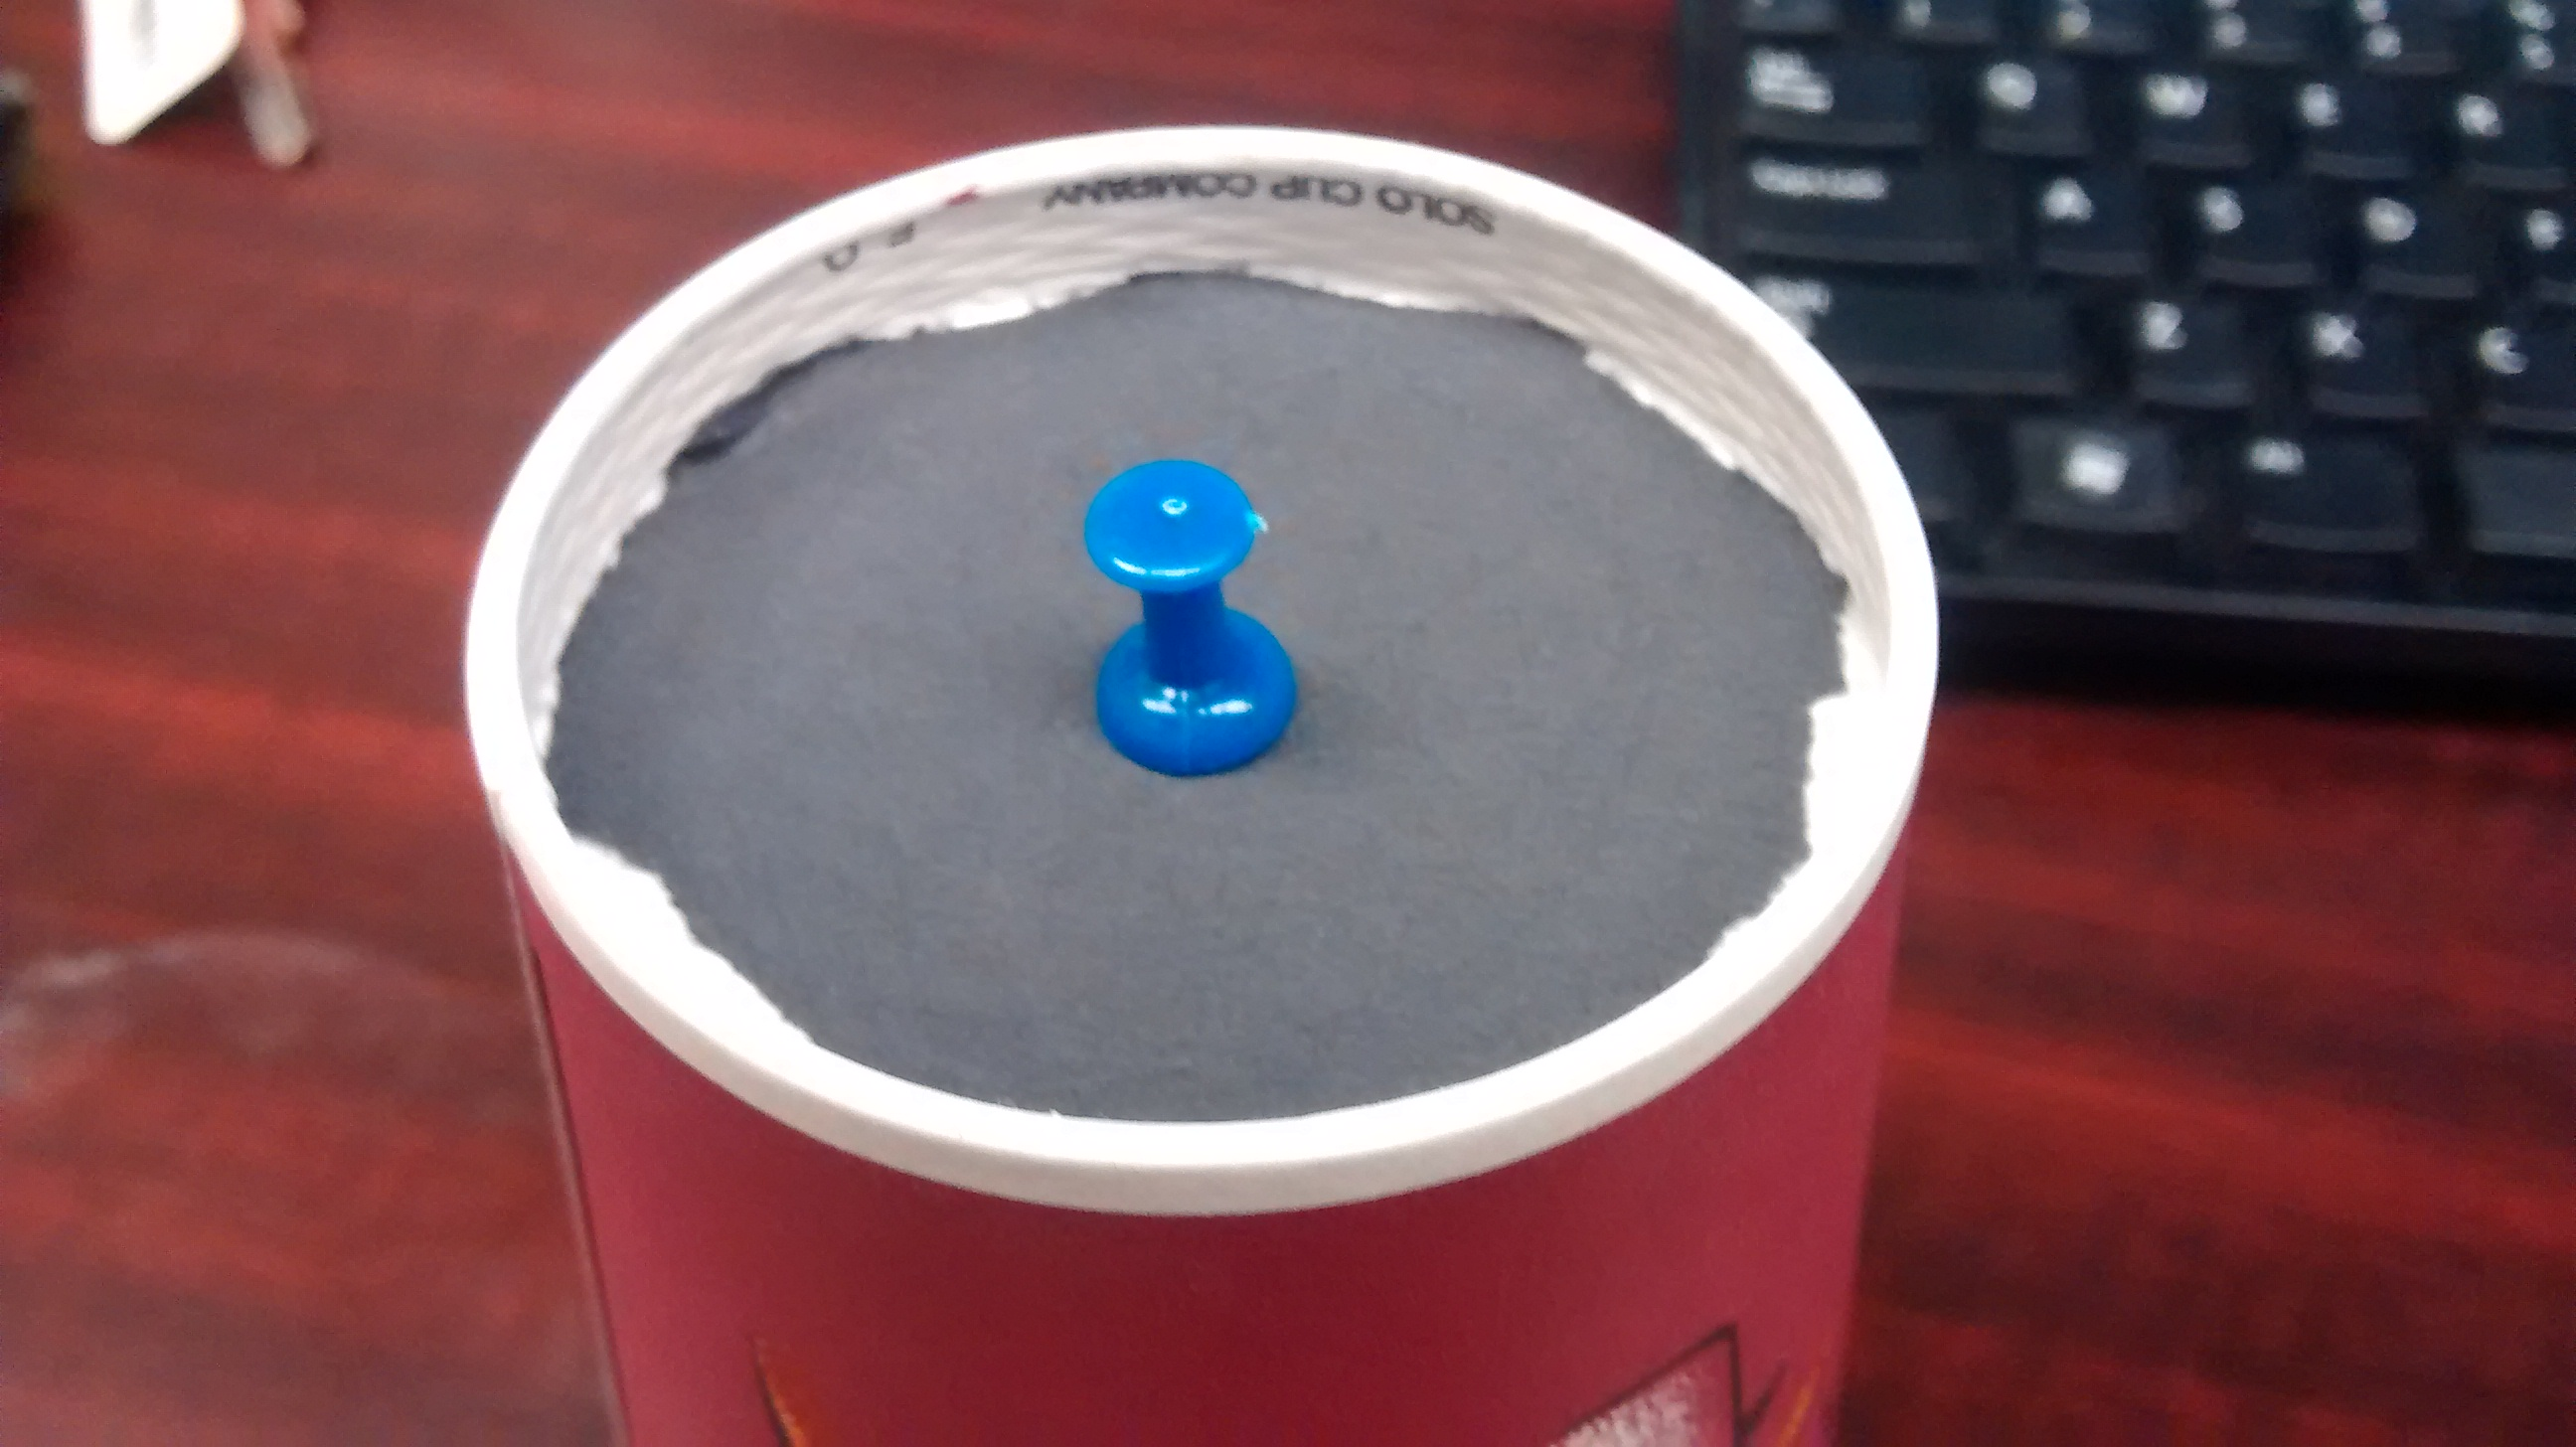
\includegraphics[width=\textwidth]{media/pushpin.jpg}
    \end{column}
  \end{columns}
\end{frame}

\begin{frame}{Pinhole camera is ready to use}
  \centering
  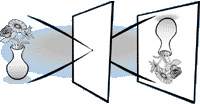
\includegraphics{media/upside_down_vase.png}
\end{frame}

\section{How does it works}

\begin{frame}{Ray diagram}
  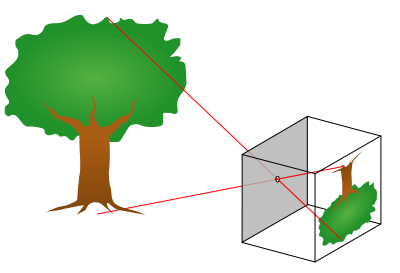
\includegraphics[width=\textwidth]{media/pinhole.png}
\end{frame}

\begin{frame}{Guess what happens?}
  ... if we make the pinhole a little bigger.\\
  \pause
  {\color{red} Image becomes brighter but blurred}
\end{frame}

\begin{frame}{Why?}
  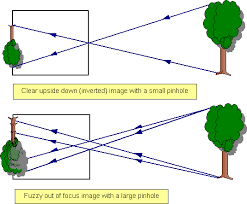
\includegraphics[width=\textwidth]{media/pinhole_blurred.png}
\end{frame}

\begin{frame}{Fun fact!!}
  \begin{center}
    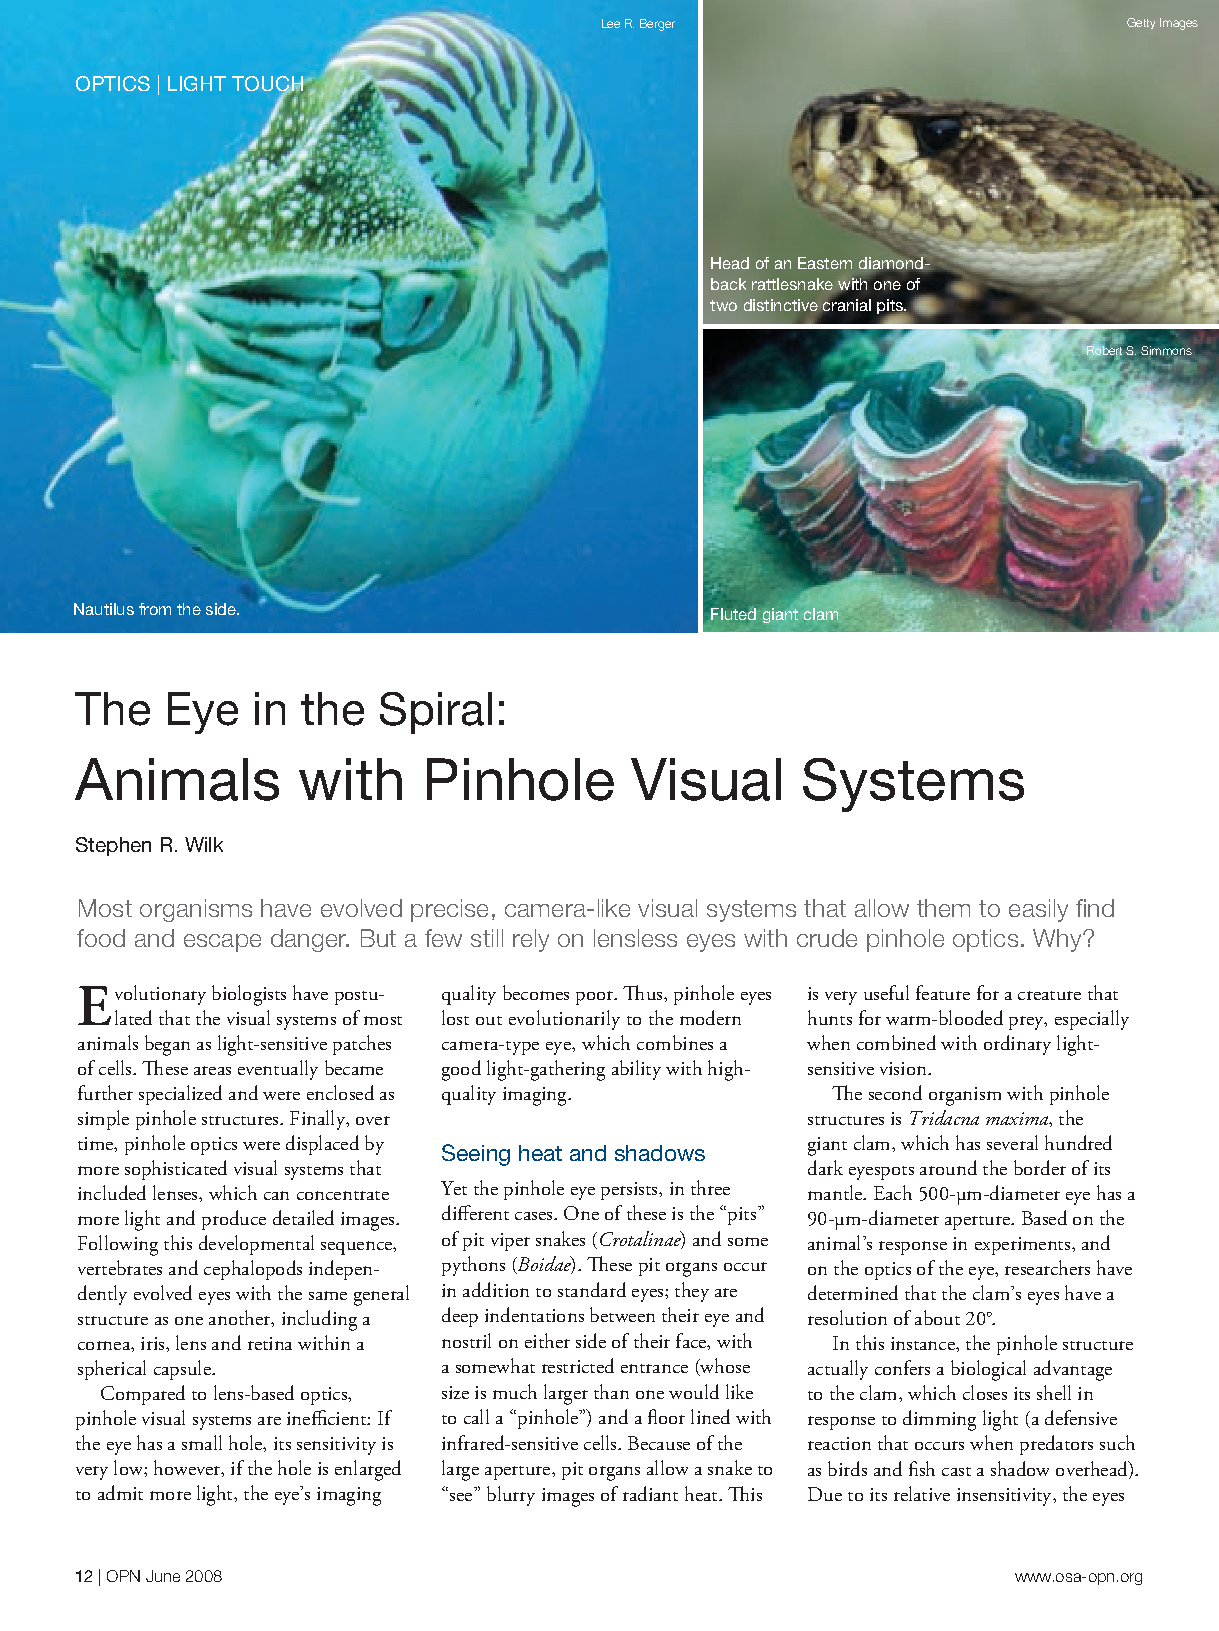
\includegraphics[width=0.8\textwidth, trim=0 5in 0 0,clip]{media/animalspinhole.pdf}
  \end{center}
\end{frame}

\begin{frame}{Evolution of eye}
  \begin{center}
  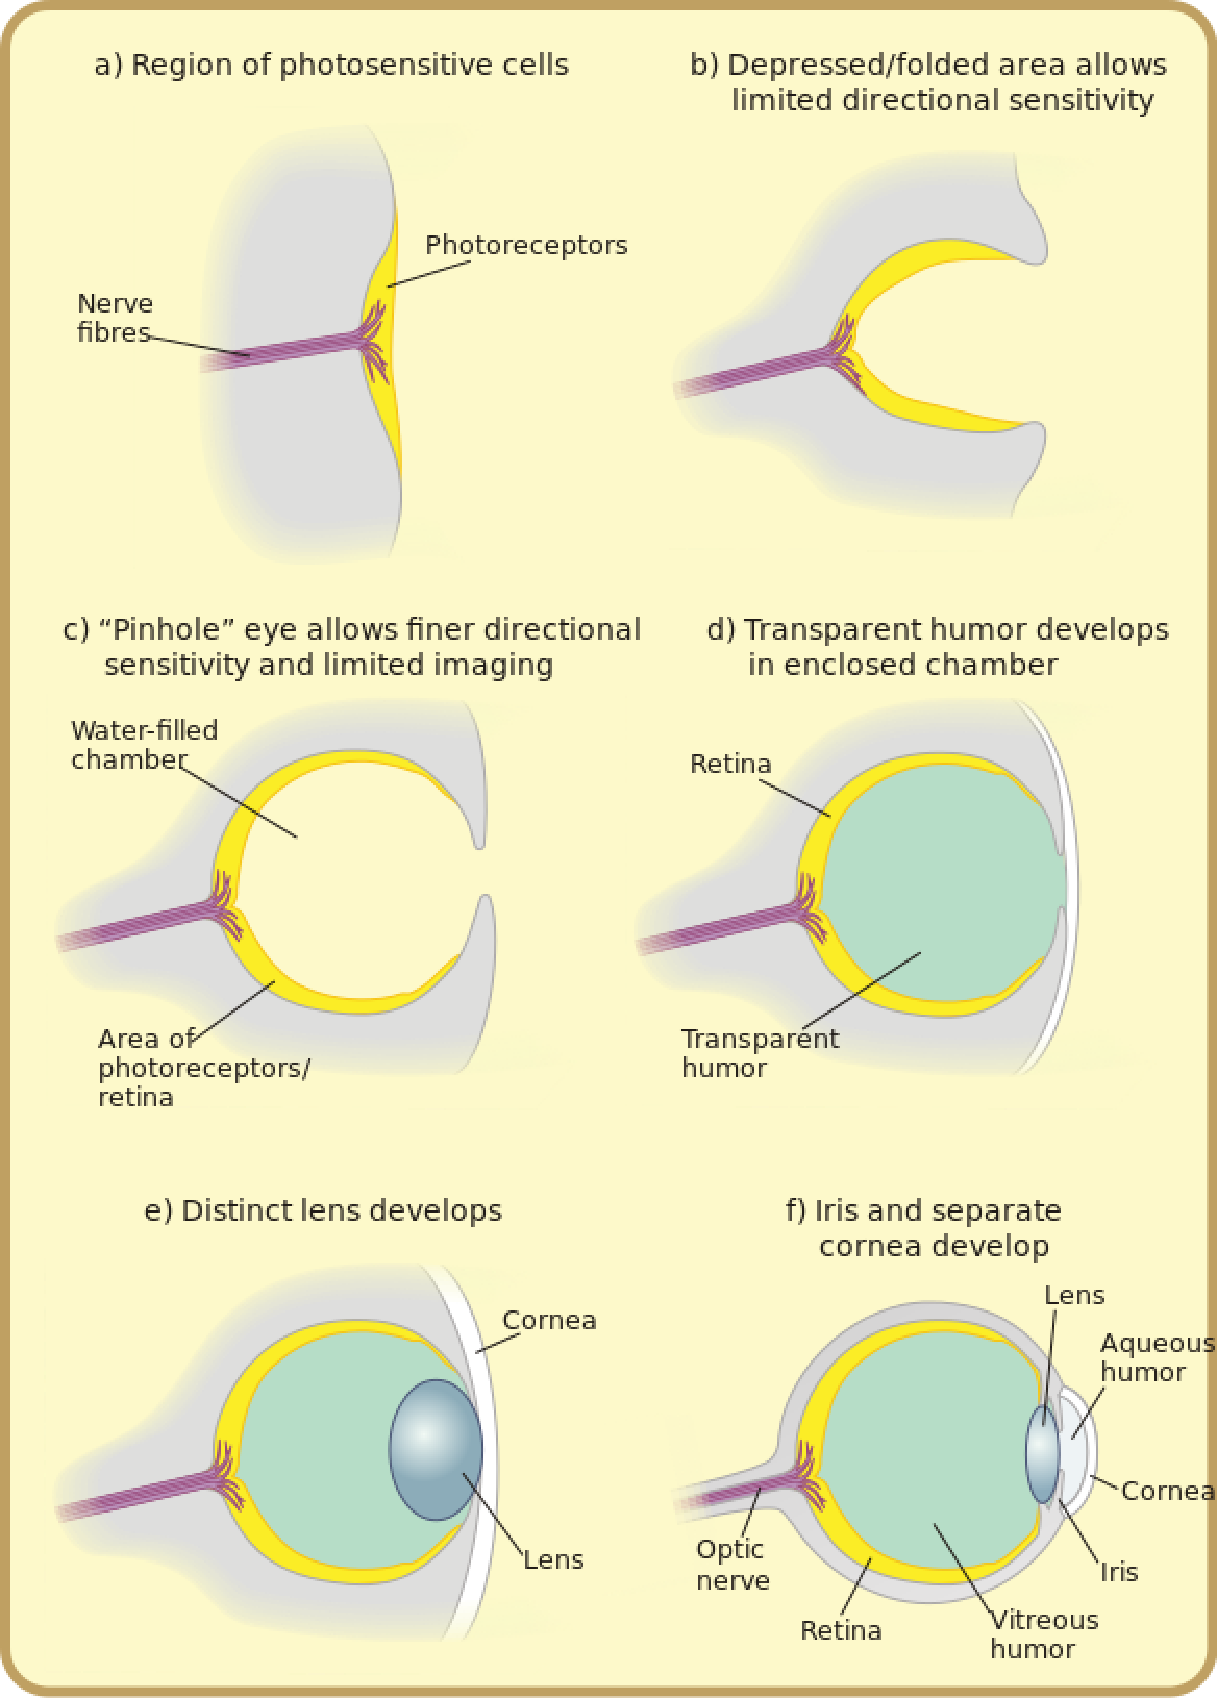
\includegraphics[height=0.8\textheight]{media/Diagram_of_eye_evolution.pdf}
  \end{center}
\end{frame}

\begin{frame}{Guess what happens}
  ... if we make multiple holes around the pinhole?\\
  \pause
  Try it ...\\
  \pause
  {\color{red} Did you get multiple images?}
\end{frame}

\begin{frame}{Guess what happens}
  ... if you change the distance of the pinhole from the object?
  \pause
  Take the camera closer to the object.
  \pause
  {\color{red} Does it become bigger?}
\end{frame}

\begin{frame}{Relating distance with image size?}
  Can you find the distance of the object given the size of object.
\end{frame}

\begin{frame}{Similar triangles}
  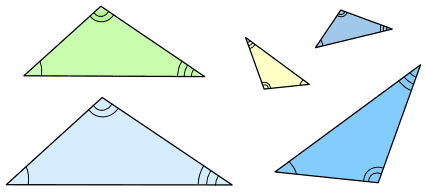
\includegraphics[width=\textwidth]{media/tri-similar1.png}
\end{frame}

\begin{frame}{Geometry of pinhole camera}
  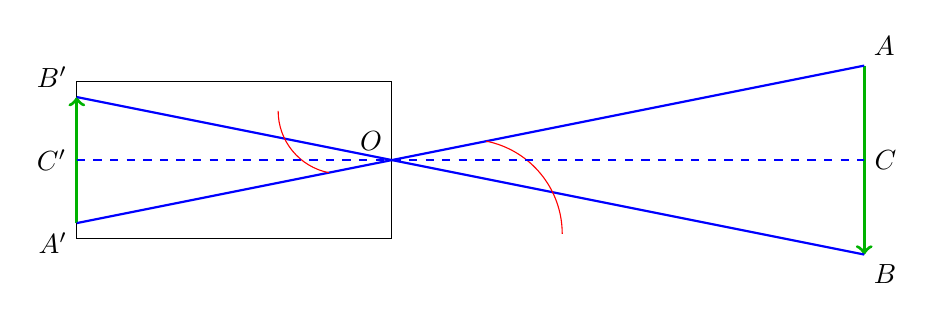
\begin{tikzpicture}
    \draw (-4,-1) rectangle (0, 1);
    \coordinate [label=above left:$O$] (origin) at (0,0);
    \coordinate [label=below left:$A'$] (imga) at (-4, -0.8);
    \coordinate [label=above left:$B'$] (imgb) at (-4, 0.8);
    \draw [->,very thick,green!70!black] (imga) -- (imgb);
    \coordinate [label=above right:$A$] (obja) at (6, 1.2);
    \coordinate [label=below right:$B$] (objb) at (6, -1.2);
    \draw [->,very thick,green!70!black] (obja) -- (objb);

    \draw [thick,blue] (imga) -- (obja);
    \draw [thick,blue] (imgb) -- (objb);
    
    \draw [red] let 
    \p1 = ($ 0.2*(imga) $),
    \n1 = {atan2(-\x1, -\y1)} 
    in (\x1,\y1) arc (\n1:0:\x1);

    \draw [red] let 
    \p1 = ($ 0.2*(obja) $),
    \n1 = {atan2(\x1, \y1)} 
    in (\x1,\y1) arc (\n1:0:\x1);

    \draw [thick,blue,dashed] ($0.5*(imga)+0.5*(imgb)$) node [text=black,anchor=east] {$C'$} -- ($0.5*(obja)+0.5*(objb)$) node [text=black,anchor=west] {$C$};
  \end{tikzpicture}
  \centering
  \begin{align}
    \frac{AC}{OC} &= \frac{A'C'}{OC'}\\
    \frac{\text{Size of object}}{\text{Distance of object}} &= \frac{\text{Size of screen}}{\text{Distance of image}}
  \end{align}
\end{frame}

\begin{frame}{Exercise}

  Can we compute the distance of object?\\
  \pause
  \begin{align}
    \text{Distance of object} = \frac{\text{Size of object}}{\text{Size of image}} \times \text{Distance of screen}
  \end{align}
\end{frame}

\begin{frame}{Recall evolution of eye}
  \begin{center}
  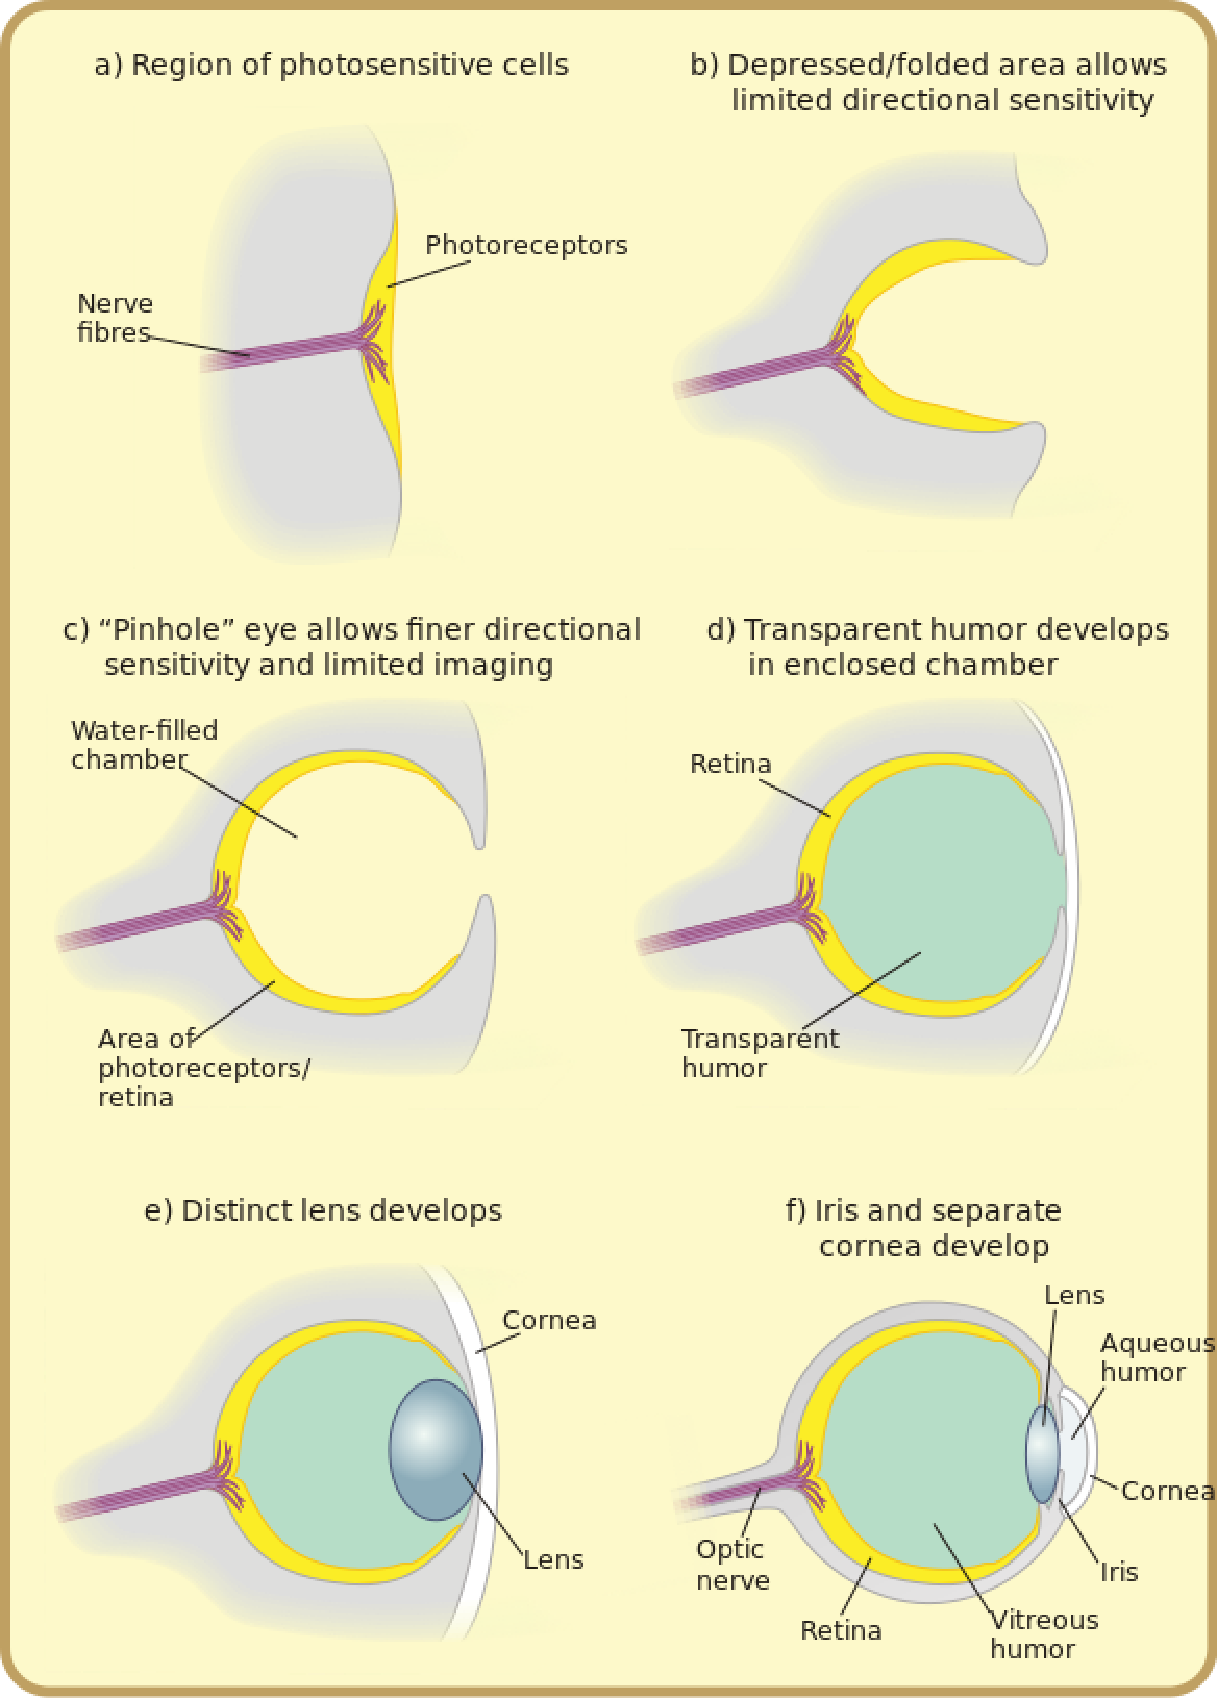
\includegraphics[height=0.8\textheight]{media/Diagram_of_eye_evolution.pdf}
  \end{center}
\end{frame}

\begin{frame}{Introducing lens}
  Add the lens in front of multiple pinholes?\\
  \pause
  Do you see all images merging into one?\\
  What happened?
\end{frame}

\begin{frame}{Understanding refraction}
  \centering
  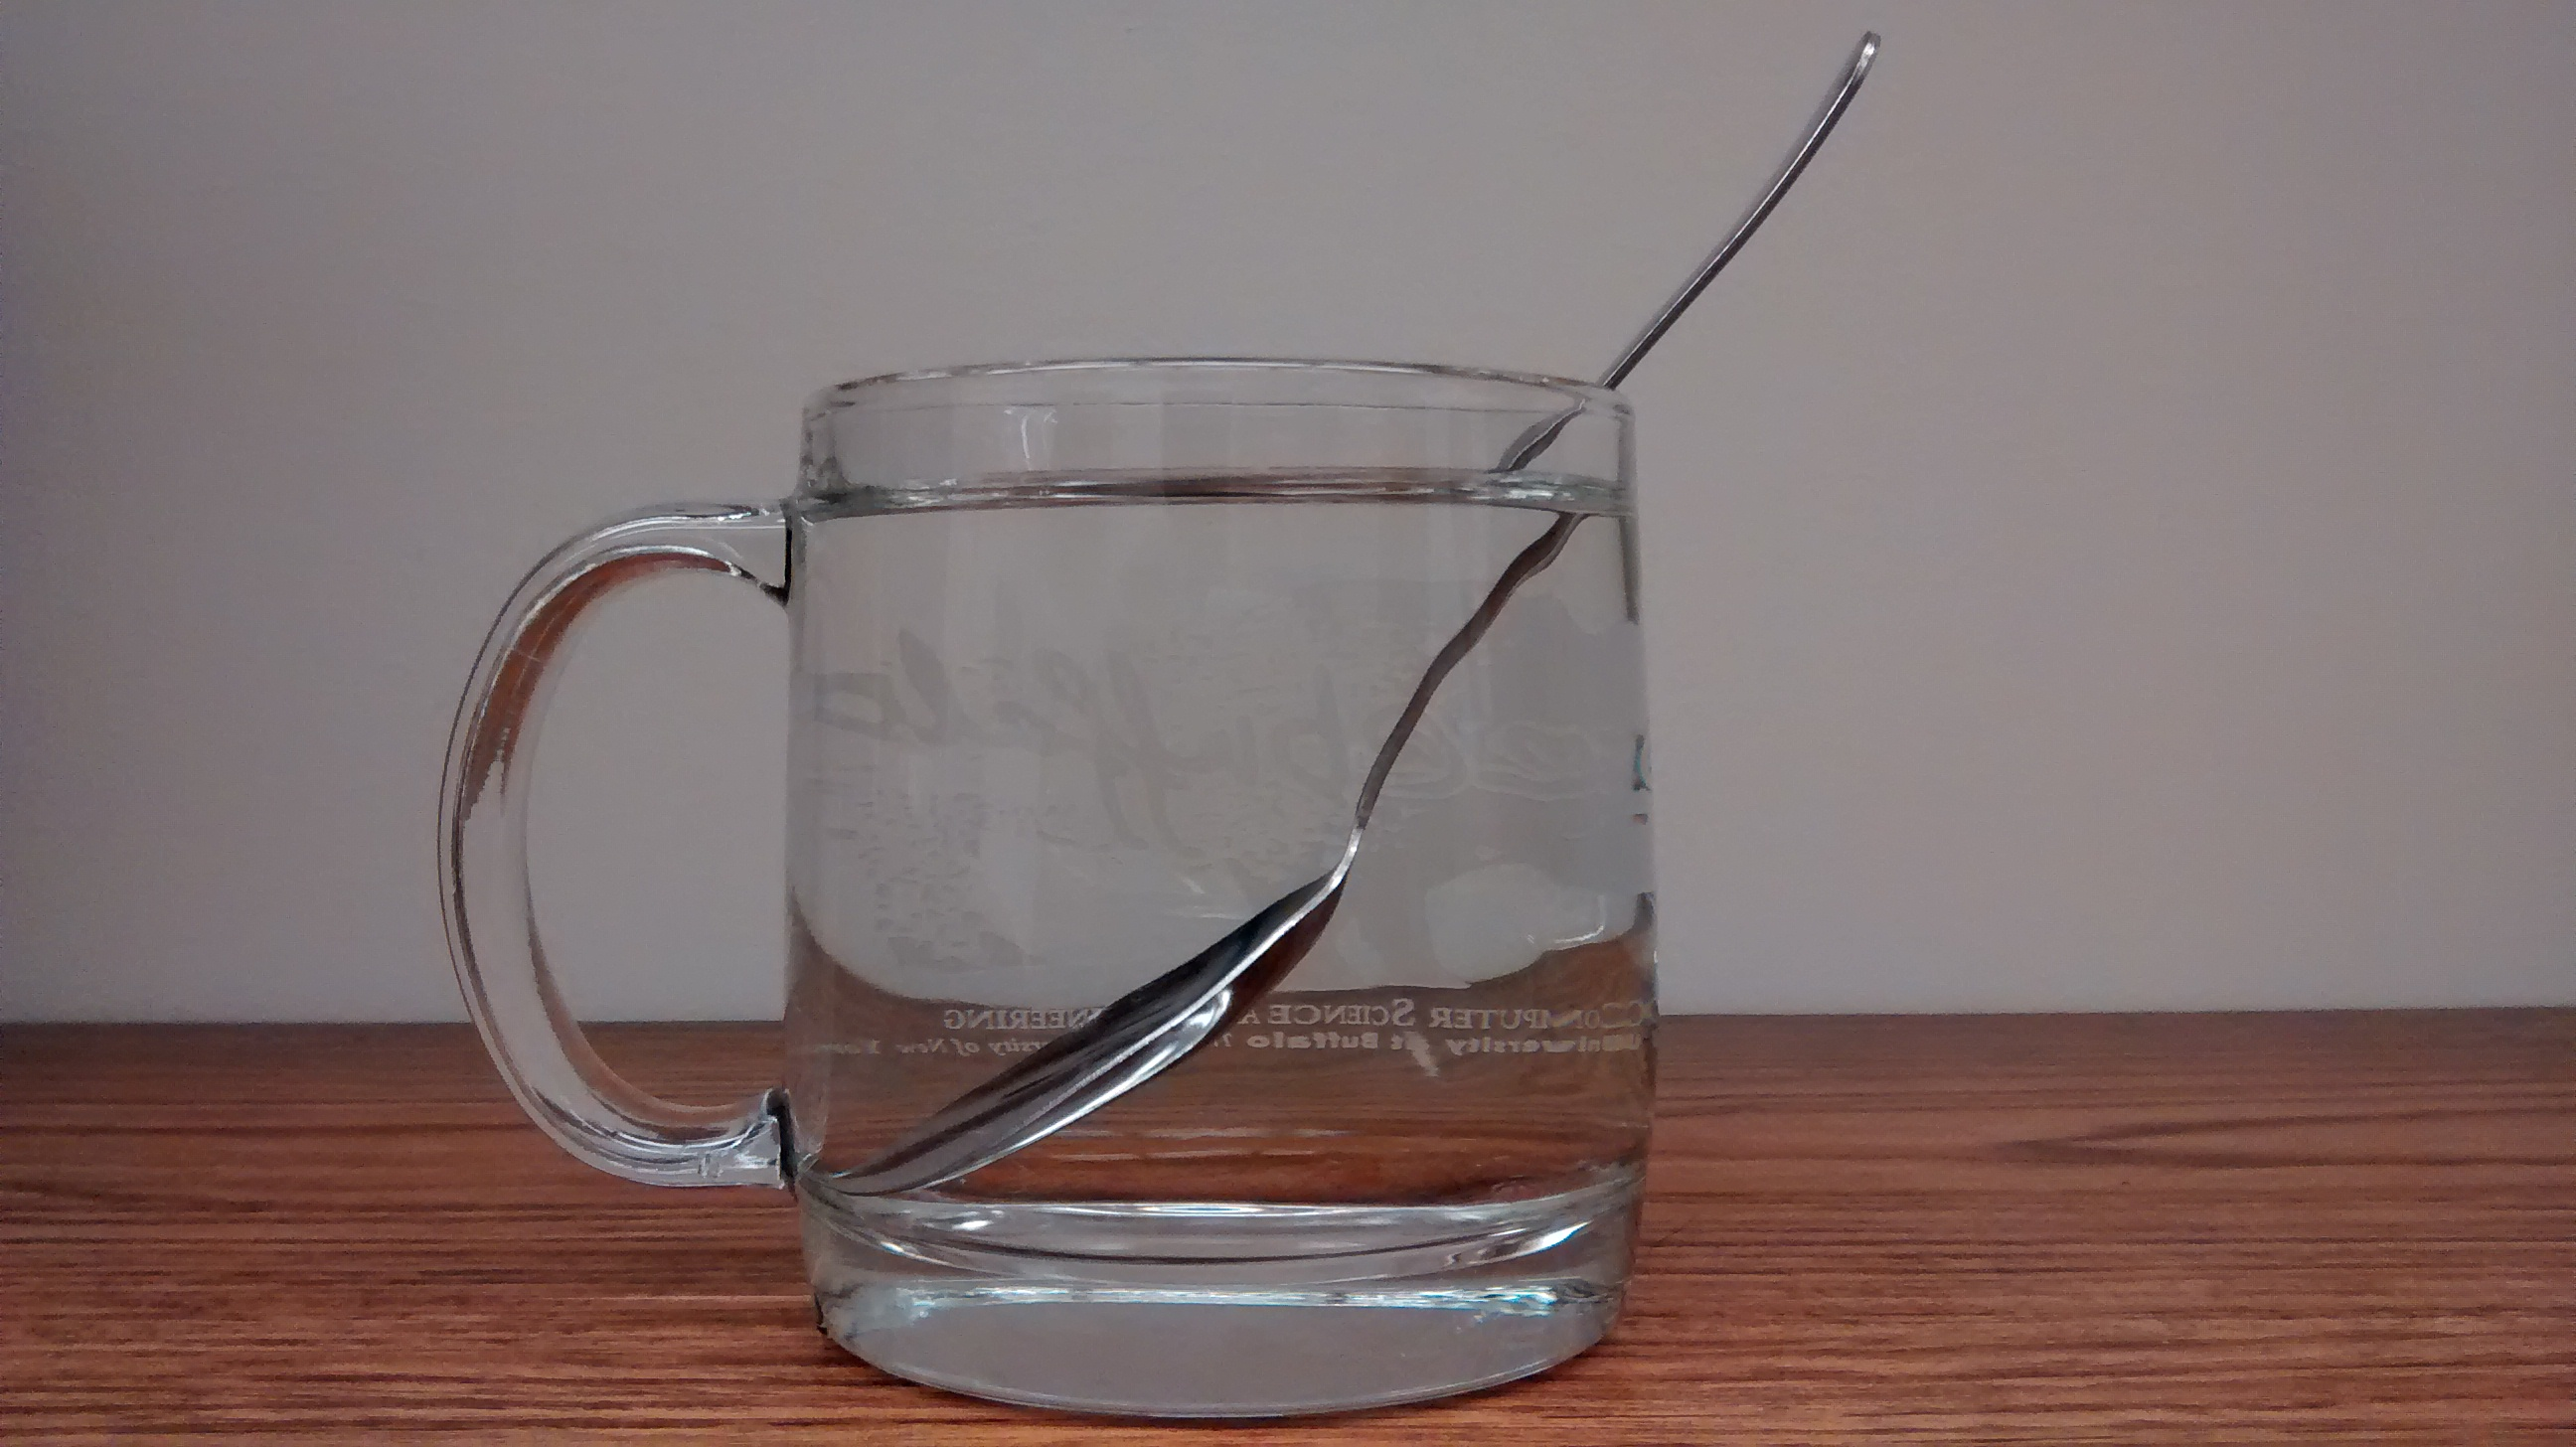
\includegraphics[width=\textwidth]{media/refractionspoon.jpg}
\end{frame}

\begin{frame}{Refraction}
  Light bends towards normal when enters a denser medium \\
  \visible<2->{
  Light bends away from normal when enters a lighter medium}
  \begin{center}
    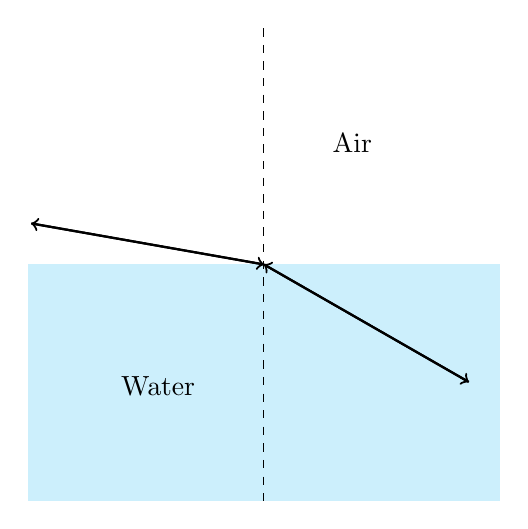
\begin{tikzpicture}[scale=3.0]
      \fill [cyan!20!white] (-1,-1) rectangle (1,0);
      \draw [dashed] (90:1) -- (-90:1);
      \visible<-1>{
        \draw [->,thick] (170:1) -- (0,0);
        \draw [->,thick] (0,0) -- (-29.84:1);
      }
      \visible<2->{
        \draw [<-,thick] (170:1) -- (0,0);
        \draw [<-,thick] (0,0) -- (-29.84:1);
      }
      \node at (60:0.5) [anchor=south west] {Air};
      \node at (-120:0.5) [anchor=north east] {Water};
    \end{tikzpicture}
  \end{center}
\end{frame}

\begin{frame}{Refraction in nature}
  Twinkling starts\\
  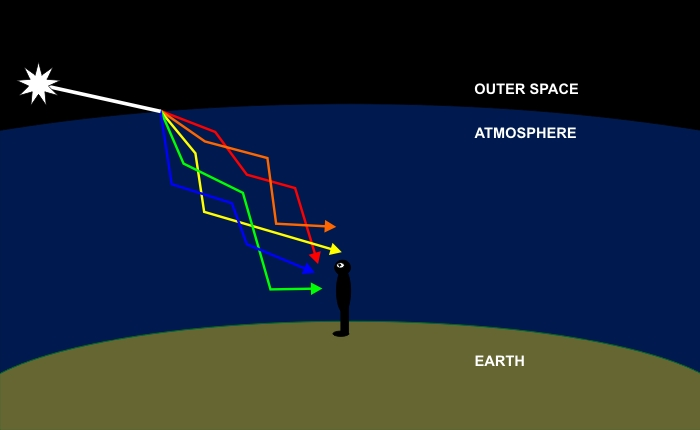
\includegraphics[width=\textwidth]{media/twinkle.jpg}
\end{frame}
\begin{frame}{Refraction in nature}
  Longer days\\
  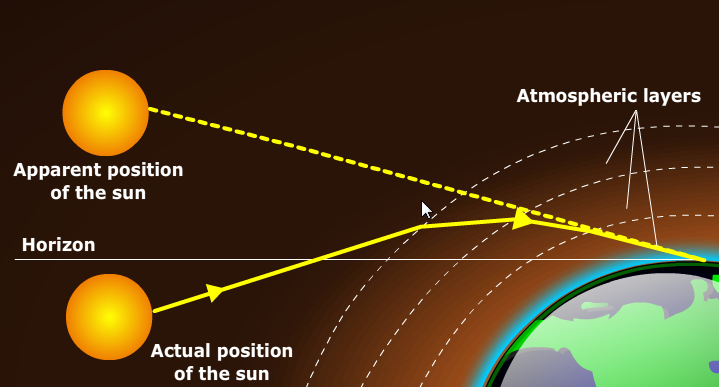
\includegraphics[width=\textwidth]{media/sunset.png}
\end{frame}

\begin{frame}{Refraction at lens}
  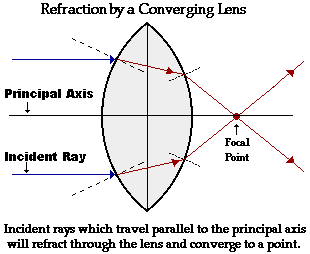
\includegraphics[height=0.8\textheight]{media/convexlens.png}
\end{frame}

\begin{frame}{Iteractive animation}

  \url{http://www.pbslearningmedia.org/resource/lsps07.sci.phys.energy.geometoptics/geometric-optics/}

\end{frame}
\end{document}
